% =====================================================================
%  Γραμμική και Συνδυαστική Βελτιστοποίηση — Βελτιστοποίηση Μενού
%  Επαυξημένη έκδοση με Δυϊκή Ανάλυση (LP Duality)
%  Μεταγλώττιση:  lualatex report.tex  (x2 για πίνακα περιεχομένων)
% =====================================================================
\documentclass[11pt,a4paper]{article}

\usepackage{amsmath,amssymb}
\usepackage{fontspec}
\usepackage{unicode-math}
\setmathfont{TeX Gyre Termes Math}
\usepackage{polyglossia}
\setmainlanguage{greek}
\setotherlanguage{english}
\setmainfont{GFS Didot}
\newcommand{\en}[1]{\textenglish{#1}}

% Διόρθωση: η αυτόματη ανίχνευση σεναρίου (script) της polyglossia δίνει εσφαλμένα
% αρνητικό αποτέλεσμα για τη γραμματοσειρά GFS Didot υπό αυτό το luaotfload — παρότι
% η γραμματοσειρά ΠΕΡΙΕΧΕΙ ελληνικά γλυφά. Παρακάμπτουμε τον έλεγχο.
\ExplSyntaxOn
\cs_set:cpn { polyglossia@addfontfeature@script:nn } #1#2 {
  \tl_if_empty:nF {#2} { \addfontfeature{Script=#2} }
}
\ExplSyntaxOff

\usepackage[a4paper,margin=2.6cm]{geometry}
\usepackage{booktabs}
\usepackage{graphicx}
\usepackage{caption}
\usepackage{array}
\usepackage{xcolor}
\usepackage{url}
\definecolor{navy}{HTML}{1F4E78}
\definecolor{linkblue}{HTML}{2456A6}

% Καλή στοίχιση ελληνικού κειμένου χωρίς διαθέσιμα πρότυπα συλλαβισμού.
\sloppy
\setlength{\emergencystretch}{3em}

\captionsetup{labelfont={bf,color=navy},font=small,labelsep=period}
\setlength{\parskip}{0.35em}
\renewcommand{\arraystretch}{1.12}

% Χρωματισμός επικεφαλίδων ενοτήτων (όπως στην αρχική αναφορά)
\usepackage{titlesec}
\titleformat{\section}{\color{navy}\Large\bfseries}{\thesection}{0.6em}{}
\titleformat{\subsection}{\color{navy}\large\bfseries}{\thesubsection}{0.6em}{}

% Μακροεντολές αριθμητικών μεγεθών παραγόμενες από τον κώδικα
\newcommand{\LPobj}{1976,41}
\newcommand{\DUALobj}{1976,41}
\newcommand{\LaborShadow}{20,37}
\newcommand{\LaborWage}{7,80}

\newcommand{\Hlow}{61,88}
\newcommand{\Hhigh}{69,35}
\newcommand{\Hdec}{3,12}
\newcommand{\Hinc}{4,35}
\newcommand{\RelaxBound}{1715,88}
\newcommand{\IntOpt}{1709,53}
\newcommand{\IntGap}{6,35}
\newcommand{\IntGapPct}{0,37}
\newcommand{\FracDishes}{Γιουβέτσι (κιμάς), Κεφτέδες}


\title{\color{navy}\bfseries\huge Γραμμική και Συνδυαστική Βελτιστοποίηση\\[0.3em]
\normalsize\mdseries\color{black} Βελτιστοποίηση Μενού Εστιατορίου με Γραμμικό\\
και Μικτό Ακέραιο Προγραμματισμό}
\author{Ευστάθιος Χρυσοβαλάντης Λιαποδημήτρης — ΑΜ 1100923}
\date{Ιούλιος 2026 \;\textit{(επαυξημένη έκδοση με δυϊκή ανάλυση)}}

\begin{document}
\maketitle
\thispagestyle{empty}

% ---------------------------------------------------------------------
\begin{abstract}
\noindent
Στην παρούσα εργασία αναπτύσσεται ένα ολοκληρωμένο υπολογιστικό σύστημα
(Python~3, βιβλιοθήκες \en{PuLP} και \en{openpyxl}, επιλύτης \en{CBC}) για τον
στρατηγικό σχεδιασμό του ημερήσιου μενού ενός εστιατορίου. Το πρόβλημα
μοντελοποιείται με δύο ανεξάρτητα μαθηματικά προγράμματα: ένα μοντέλο
\emph{Γραμμικού Προγραμματισμού} (\en{LP}) που δίνει το θεωρητικό άνω φράγμα του
κέρδους, και ένα μοντέλο \emph{Μικτού Ακέραιου Προγραμματισμού} (\en{MIP}) που
παράγει ένα \emph{υλοποιήσιμο} μενού με πεπερασμένο πλήθος πιάτων και πάγια κόστη
προετοιμασίας. Παρουσιάζονται αναλυτικά η βάση δεδομένων (52 πρώτες ύλες, 21
συνταγές) μαζί με τις πηγές των τιμών, η ακριβής κοστολόγηση κάθε πιάτου, η δομή
των δύο μοντέλων, η σχέση τους, καθώς και εκτενής ανάλυση ευαισθησίας. Η ανάλυση
εμβαθύνει με πλήρη \emph{δυϊκή ανάλυση} του \en{LP} (Ενότητα~\ref{sec:duality}):
διατυπώνεται ρητά το δυϊκό πρόβλημα, επιβεβαιώνεται αριθμητικά η \emph{ισχυρή
δυϊκότητα} ($Z^\star=W^\star=\LPobj$\,€), και ερμηνεύονται οι \emph{σκιώδεις τιμές}
και τα \emph{μειωμένα κόστη}. Ακολουθεί \emph{παραμετρική ανάλυση και εύρος
ευστάθειας} (Ενότητα~\ref{sec:ranging}) και μελέτη του \emph{διακένου ακεραιότητας}
του \en{branch \& bound} (Ενότητα~\ref{sec:bnb}). Έτσι το κεντρικό ερώτημα — γιατί ορισμένα
παραδοσιακά πιάτα μένουν εκτός μενού — απαντάται πλέον \emph{αυστηρά} μέσω του
κόστους ευκαιρίας: η σκιώδης τιμή της εργασίας ($u^\star=\LaborShadow$\,€/ώρα)
υπερβαίνει κατά πολύ το ωρομίσθιο (\LaborWage\,€/ώρα), οπότε κάθε λεπτό
αφιερωμένο σε αργό πιάτο κοστίζει περισσότερο απ' όσο αποδίδει.
\end{abstract}

\tableofcontents
\newpage

% =====================================================================
\section{Εισαγωγή και Περιγραφή του Προβλήματος}
Ο σχεδιασμός του μενού ενός εστιατορίου αποτελεί ένα κλασικό πρόβλημα κατανομής
περιορισμένων πόρων. Ο διαχειριστής καλείται να απαντήσει ταυτόχρονα σε τρία
ερωτήματα:
\begin{enumerate}
  \item \textbf{Ποια πιάτα} θα προσφέρει το εστιατόριο σήμερα;
  \item \textbf{Πόσες μερίδες} θα παραχθούν από κάθε πιάτο;
  \item \textbf{Πώς} κατανέμεται ο διαθέσιμος χρόνος του προσωπικού ανάμεσα στα πιάτα;
\end{enumerate}

Οι αποφάσεις αυτές δεν είναι ανεξάρτητες. Κάθε πιάτο δεσμεύει συγκεκριμένο χρόνο
κουζίνας, καταναλώνει πρώτες ύλες με δεδομένο κόστος, και μπορεί να πουληθεί μόνο
μέχρι ένα άνω όριο ζήτησης της αγοράς. Στόχος αποτελεί η
\textbf{μεγιστοποίηση του ημερήσιου μεικτού κέρδους}, δηλαδή των εσόδων μείον του
μεταβλητού κόστους (υλικά, εργασία, σπατάλη) και --- στο δεύτερο μοντέλο --- μείον
των πάγιων κοστών προετοιμασίας των πιάτων που τελικά εντάσσονται στο μενού.

Μεθοδολογικά, το πρόβλημα ανήκει στην παράδοση του \emph{Γραμμικού
Προγραμματισμού}, όπως θεμελιώθηκε από τον \en{Dantzig}~\cite{dantzig}, και
συγγενεύει άμεσα με το ιστορικό \emph{πρόβλημα διατροφής} (\en{diet problem}) του
\en{Stigler}~\cite{stigler}. Η θεωρία της \emph{δυϊκότητας} και της ανάλυσης
ευαισθησίας που αξιοποιούμε στις Ενότητες~\ref{sec:duality}--\ref{sec:ranging}
ακολουθεί τα καθιερωμένα εγχειρίδια~\cite{bertsimas,winston}, ενώ η επίλυση του
ακέραιου μοντέλου βασίζεται στη μέθοδο \emph{branch \& bound}~\cite{landdoig,wolsey}.

\paragraph{Δομή της εργασίας.} Στην Ενότητα~\ref{sec:data} παρουσιάζεται αναλυτικά
η βάση δεδομένων, οι πηγές των τιμών και ο τρόπος με τον οποίο παράγεται από αυτήν
η κοστολόγηση κάθε πιάτου. Στην Ενότητα~\ref{sec:model} αναπτύσσονται τα δύο
μαθηματικά μοντέλα και αποσαφηνίζεται η μεταξύ τους σχέση. Στην
Ενότητα~\ref{sec:results} ερμηνεύονται τα αποτελέσματα, ενώ η
Ενότητα~\ref{sec:duality} εμβαθύνει με τη \emph{δυϊκή θεωρία} και η
Ενότητα~\ref{sec:ranging} με την \emph{παραμετρική ανάλυση και το εύρος ευστάθειας}.
Η Ενότητα~\ref{sec:sensitivity} περιέχει την ανάλυση ευαισθησίας, στην
Ενότητα~\ref{sec:discussion} συζητούνται κριτικά τα ευρήματα, και τα συμπεράσματα
συνοψίζονται στην Ενότητα~\ref{sec:conclusions}.

\subsection{Σχέση με τη βιβλιογραφία}\label{sec:literature}
Το πρόβλημα εντάσσεται στην ευρύτερη οικογένεια προβλημάτων \emph{σχεδιασμού μενού}
(\en{menu planning}) και του κλασικού \emph{προβλήματος διατροφής} (\en{diet
problem}). Το τελευταίο διατυπώθηκε από τον \en{Stigler}~\cite{stigler} το 1945 και
έγινε ένα από τα πρώτα μεγάλα προβλήματα που επιλύθηκαν με τη μέθοδο \en{simplex}
του \en{Dantzig}~\cite{dantzig}· έκτοτε αποτελεί υπόδειγμα εφαρμογής Γραμμικού και
Ακέραιου Προγραμματισμού. Παρακάτω αναλύονται τρεις \emph{σύγχρονες} εργασίες
αναφοράς --- η καθεμία αντιπροσωπευτική μιας διαφορετικής μεθοδολογικής επιλογής ---
και οριοθετείται τι αντλεί και τι διαφοροποιεί η παρούσα υλοποίηση.

\paragraph{\en{Razak et al.}~\cite{razak} — Γραμμικός Προγραμματισμός στο \en{Diet Problem}.}
Η εργασία εφαρμόζει το κλασικό πρόβλημα διατροφής σε πραγματικά είδη μενού μιας
αλυσίδας εστίασης (\en{Kenny Rogers Roasters}). Χρησιμοποιεί \emph{συνεχείς}
μεταβλητές και \emph{ελαχιστοποιεί το κόστος} ενός γεύματος υπό την προϋπόθεση ότι
καλύπτονται οι ημερήσιες διατροφικές απαιτήσεις (θερμίδες, πρωτεΐνη, λιπαρά κ.λπ.),
οι οποίες εκφράζονται ως γραμμικοί περιορισμοί. Είναι η πιο «καθαρά \en{LP}» από
τις τρεις προσεγγίσεις. \emph{Αντλούμε} από αυτήν τη διατύπωση συνεχούς γραμμικού
προγράμματος πόρων (Μοντέλο Α, Ενότητα~\ref{sec:model})· \emph{διαφοροποιούμαστε}
αντιστρέφοντας τον στόχο (μεγιστοποίηση κέρδους αντί ελαχιστοποίησης κόστους) και
αντικαθιστώντας τον διατροφικό προϋπολογισμό με τον περιορισμό εργατοωρών.

\paragraph{\en{Sholeha et al.}~\cite{sholeha} — \en{Boolean / Integer Linear Programming} για \en{Diet-Menu}.}
Η εργασία μοντελοποιεί τη σύνθεση ενός διαιτολογίου με \emph{δυαδικές} (0--1)
μεταβλητές: για κάθε υποψήφιο έδεσμα μια μεταβλητή αποφασίζει αν αυτό θα
συμπεριληφθεί ή όχι. Πρόκειται για Ακέραιο/\en{Boolean} Πρόγραμμα όπου
ελαχιστοποιείται το κόστος υπό διατροφικές ανάγκες. \emph{Αντλούμε} ακριβώς το
στοιχείο της \emph{δυαδικής μεταβλητής επιλογής} $y_d\in\{0,1\}$ (Μοντέλο Β,
σχέσεις~\eqref{eq:miplink}--\eqref{eq:mipmin})· \emph{διαφοροποιούμαστε} συνδέοντάς
την με \emph{πάγια κόστη ένταξης} και με συνεχείς ποσότητες παραγωγής $x_d$ ---
δηλαδή \emph{μικτό} και όχι αμιγώς δυαδικό πρόγραμμα.

\paragraph{\en{Silva et al.}~\cite{silva} — \en{Integer Linear Programming} για μενού πανεπιστημιακών εστιατορίων.}
Η εργασία σχεδιάζει (συχνά κυκλικά/εβδομαδιαία) μενού φοιτητικών εστιατορίων με
\en{ILP}, επιλέγοντας εδέσματα υπό διατροφικούς περιορισμούς, περιορισμούς
προϋπολογισμού και --- σημαντικό για την παρούσα εργασία --- περιορισμούς
\emph{ποικιλίας/πλήθους} (πόσα και τι είδους πιάτα θα υπάρχουν στο μενού).
\emph{Αντλούμε} τον περιορισμό πληθικότητας $N_{\min}\le\sum_d y_d\le N_{\max}$
(σχέση~\eqref{eq:mipsize})· \emph{διαφοροποιούμαστε} αντιμετωπίζοντάς τον ως
\emph{σχεδιαστική} παράμετρο, της οποίας την επίδραση αποτιμούμε ρητά
(Ενότητα~\ref{sec:sensitivity}).

\paragraph{Τι ακολουθεί και τι διαφοροποιεί η παρούσα εργασία.}
Από τη μεθοδολογική «εργαλειοθήκη» των παραπάνω αντλούνται τρία στοιχεία: (i)~η
διατύπωση μεγιστοποίησης/ελαχιστοποίησης γραμμικής αντικειμενικής υπό γραμμικούς
περιορισμούς πόρων με συνεχείς μεταβλητές (\en{Razak et al.}~\cite{razak})· (ii)~η
δυαδική μεταβλητή επιλογής $y_d\in\{0,1\}$ για την ένταξη ή μη ενός πιάτου
(\en{Sholeha et al.}~\cite{sholeha})· και (iii)~ο περιορισμός πληθικότητας του μενού
$N_{\min}\le\sum_d y_d\le N_{\max}$ (\en{Silva et al.}~\cite{silva}). Η ουσιαστική
διαφοροποίηση συνοψίζεται στον
Πίνακα~\ref{tab:lit}: η οπτική γωνία είναι του \emph{παραγωγού} (κερδοφορία) και
όχι του \emph{καταναλωτή} (διατροφή)· ο στενός πόρος δεν είναι διατροφικός ή
χρηματικός προϋπολογισμός αλλά ο \emph{χρόνος εργασίας} της κουζίνας· και
προστίθενται τρία στοιχεία που δεν εμφανίζονται στα παραπάνω: ρητός όρος
\emph{κόστους σπατάλης} τροφίμων, \emph{πάγια κόστη} προετοιμασίας ανά πιάτο, και
ο σχεδιασμός \emph{δύο επιπέδων} (\en{LP} ως άνω φράγμα — \en{MIP} ως υλοποιήσιμη
λύση) με ερμηνεία των σκιωδών τιμών.

\begin{table}[htbp]
\centering
\caption{Σύγκριση της παρούσας εργασίας με τη βιβλιογραφία αναφοράς.}
\label{tab:lit}
\small
\begin{tabular}{@{}p{3.1cm}p{5.0cm}p{5.5cm}@{}}
\toprule
\textbf{Διάσταση} & \textbf{Βιβλιογραφία (\en{diet}/\en{menu planning})} & \textbf{Παρούσα εργασία}\\
\midrule
Οπτική γωνία & Καταναλωτής / διατροφή & Επιχείρηση / κερδοφορία\\
Αντικειμενικός στόχος & Ελαχιστοποίηση κόστους & Μεγιστοποίηση κέρδους\\
Κύριοι περιορισμοί & Διατροφικές απαιτήσεις, προϋπολογισμός & Εργατοώρες, ζήτηση αγοράς, σπατάλη, πάγια κόστη, πλήθος πιάτων\\
Μεταβλητές & Συνεχείς \en{LP} (\en{Razak}) ή δυαδικές 0--1 \en{ILP} (\en{Sholeha}, \en{Silva}) & Και τα δύο: \en{LP} (συνεχές, άνω φράγμα) και \en{MIP} (συνεχείς + δυαδικές)\\
Στενός πόρος & Διατροφικός/χρηματικός προϋπολογισμός & Χρόνος εργασίας κουζίνας\\
Επιπλέον στοιχεία & --- & Κόστος σπατάλης, πάγια κόστη ένταξης, \textbf{δυϊκή ανάλυση} (σκιώδεις τιμές, μειωμένα κόστη)\\
\bottomrule
\end{tabular}
\end{table}

% =====================================================================
\section{Η Βάση Δεδομένων}\label{sec:data}
Η βάση δεδομένων (αρχείο \en{data.py}) περιλαμβάνει \textbf{52 πρώτες ύλες} και
\textbf{21 υποψήφια πιάτα} ελληνικής κουζίνας. Τα οικονομικά στοιχεία αφορούν το
έτος 2026.

\subsection{Πηγές των τιμών}
Οι τιμές των πρώτων υλών συγκεντρώθηκαν την περίοδο Ιανουαρίου--Μαΐου 2026 από
επίσημες πηγές και τιμοληψίες. Κάθε τιμή του Πίνακα~\ref{tab:ingredients}
αντιστοιχεί στο \emph{μέσο} ενός εύρους τιμών που παρατηρήθηκε στις παρακάτω πηγές:
\begin{itemize}
  \item \textbf{ΟΚΑΑ Α.Ε.} (Κεντρική Αγορά Αθηνών) — ημερήσια δελτία τιμών
        χονδρικής κρεάτων, λαχανικών και αλιευμάτων: \url{https://www.okaa.gr}
  \item \textbf{Παρατηρητήριο Τιμών / e-Καταναλωτής} (Υπ.\ Ανάπτυξης):
        \url{https://e-katanalotis.gov.gr}
  \item \textbf{Ηλεκτρονικά καταστήματα αλυσίδων σουπερμάρκετ}: ΑΒ Βασιλόπουλος,
        Σκλαβενίτης, \en{My Market}.
\end{itemize}
Η αντιστοίχιση κάθε κατηγορίας υλικών στην κύρια πηγή της δίνεται στον
Πίνακα~\ref{tab:sources}.

\begin{table}[htbp]
\centering
\caption{Κύρια πηγή τιμών ανά κατηγορία πρώτης ύλης.}
\label{tab:sources}
\small
\begin{tabular}{@{}ll@{}}
\toprule
\textbf{Κατηγορία} & \textbf{Κύρια πηγή}\\
\midrule
Κρέατα (κιμάδες, κοτόπουλο, παϊδάκια) & ΟΚΑΑ (χονδρική)\\
Θαλασσινά (γαρίδες, χταπόδι) & Σ/Μ (λιανική) / ΟΚΑΑ (ιχθυόσκαλα)\\
Λαχανικά \& φρούτα & Σ/Μ διασταυρωμένα με Παρατηρητήριο Τιμών\\
Δημητριακά, ζυμαρικά, όσπρια, κονσέρβες & Σ/Μ\\
Γαλακτοκομικά \& τυριά & Σ/Μ\\
Ελαιόλαδο, βασικά, μυρωδικά & Σ/Μ (λιανική)\\
\bottomrule
\end{tabular}
\end{table}

\subsection{Παράμετροι του συστήματος}
Οι καθολικές παράμετροι του προβλήματος (πίνακας \en{PARAMS}) δίνονται στον
Πίνακα~\ref{tab:params}. Αποτελούν \emph{σχεδιαστικές επιλογές} του διαχειριστή
και, όπως αναδεικνύεται στη συνέχεια, ορισμένες από αυτές (ιδίως οι διαθέσιμες
εργατοώρες $H$ και το μέγιστο πλήθος πιάτων $N_{\max}$) καθορίζουν σε μεγάλο βαθμό
τη μορφή της λύσης.

\begin{table}[htbp]
\centering
\caption{Καθολικές παράμετροι του μοντέλου.}
\label{tab:params}
\small
\begin{tabular}{@{}lcr@{}}
\toprule
\textbf{Παράμετρος} & \textbf{Σύμβολο} & \textbf{Τιμή}\\
\midrule
Διαθέσιμες εργατοώρες / ημέρα & $H$ & 65,0 ώρες\\
Ωρομίσθιο προσωπικού & $w$ & 7,80 €/ώρα\\
Ποσοστό σπατάλης υλικών & $\alpha$ & 6\%\\
Συντελεστής ποινής σπατάλης & $\beta$ & 1,0\\
Μέγιστο πλήθος πιάτων στο μενού & $N_{\max}$ & 10\\
Ελάχιστο πλήθος πιάτων στο μενού & $N_{\min}$ & 6\\
\bottomrule
\end{tabular}
\end{table}

\subsection{Πρώτες ύλες}
Κάθε πρώτη ύλη χαρακτηρίζεται από το μοναδιαίο κόστος προμήθειας (σε € ανά kg, ανά
L για τα υγρά, ή ανά τεμάχιο για τα αυγά). Ο Πίνακας~\ref{tab:ingredients}
παραθέτει το πλήρες σύνολο των 52 υλικών ανά κατηγορία.

\begin{table}[htbp]
\centering
\caption{Πρώτες ύλες — μοναδιαίο κόστος προμήθειας (μέσες τιμές 2026).}
\label{tab:ingredients}
\footnotesize
\begin{minipage}[t]{0.49\textwidth}\centering
\setlength{\tabcolsep}{4pt}
\begin{tabular}{@{}p{5.2cm}cr@{}}
\toprule
\textbf{Πρώτη ύλη} & \textbf{Μον.} & \textbf{€} \\
\midrule
\multicolumn{3}{@{}l}{\textbf{Κρέατα \& πρωτεΐνες}}\\
\quad Κιμάς μοσχαρίσιος & kg & 15,50 \\
\quad Κιμάς χοιρινός & kg & 12,00 \\
\quad Κοτόπουλο (φιλέτο/μπούτι) & kg & 12,50 \\
\quad Παϊδάκια αρνίσια (κατεψυγμένα) & kg & 12,50 \\
\addlinespace
\multicolumn{3}{@{}l}{\textbf{Θαλασσινά}}\\
\quad Γαρίδες κατεψυγμένες (Νο 2) & kg & 14,00 \\
\quad Χταπόδι κατεψυγμένο & kg & 13,00 \\
\addlinespace
\multicolumn{3}{@{}l}{\textbf{Λαχανικά φρέσκα}}\\
\quad Πατάτες & kg & 0,80 \\
\quad Ντομάτα φρέσκια (κόκκινη) & kg & 1,80 \\
\quad Ντομάτα κεράσι (cherry) & kg & 3,50 \\
\quad Μελιτζάνες & kg & 2,20 \\
\quad Πιπεριές κόκκινες/πράσινες & kg & 3,00 \\
\quad Κρεμμύδια ξερά & kg & 1,10 \\
\quad Κρεμμύδια verde (φρέσκα) & kg & 4,50 \\
\quad Σπανάκι φρέσκο & kg & 2,50 \\
\quad Σκόρδο & kg & 6,00 \\
\quad Μπάμια & kg & 3,20 \\
\quad Κολοκιθάκια & kg & 1,90 \\
\quad Αγκινάρες & kg & 2,80 \\
\quad Πορτοκάλια & kg & 1,50 \\
\quad Λεμόνια & kg & 1,80 \\
\addlinespace
\multicolumn{3}{@{}l}{\textbf{Δημητριακά \& αμυλούχα}}\\
\quad Ρύζι (Καρολίνα) & kg & 1,60 \\
\quad Ρύζι Arborio (risotto) & kg & 2,80 \\
\quad Μακαρόνια (No6) & kg & 1,30 \\
\quad Χηλοπίτες (φύλλο ζύμης) & kg & 1,50 \\
\quad Αλεύρι (Τύπου 550) & kg & 1,20 \\
\quad Κορνάρι ψωμιού & kg & 2,50 \\
\quad Ψωμί (κατάλληλο για κρούμπες) & kg & 1,00 \\
\addlinespace
\bottomrule
\end{tabular}

\end{minipage}\hfill
\begin{minipage}[t]{0.49\textwidth}\centering
\setlength{\tabcolsep}{4pt}
\begin{tabular}{@{}p{5.2cm}cr@{}}
\toprule
\textbf{Πρώτη ύλη} & \textbf{Μον.} & \textbf{€} \\
\midrule
\multicolumn{3}{@{}l}{\textbf{Γαλακτοκομικά}}\\
\quad Φέτα ΠΟΠ & kg & 11,00 \\
\quad Γραβιέρα ΠΟΠ & kg & 14,50 \\
\quad Κεφαλοτύρι ΠΟΠ (τριμμένο) & kg & 13,00 \\
\quad Μανούρι & kg & 12,50 \\
\quad Γάλα φρέσκο (3,6\% λιπαρά) & L & 1,35 \\
\quad Βούτυρο & kg & 9,00 \\
\quad Αυγά (τεμάχιο) & τεμ & 0,30 \\
\quad Γιαούρτι στραγγιστό & L & 1,20 \\
\quad Μυζήθρα & kg & 8,50 \\
\addlinespace
\multicolumn{3}{@{}l}{\textbf{Βασικά \& μυρωδικά}}\\
\quad Ελαιόλαδο έξτρα παρθένο & L & 7,00 \\
\quad Αλάτι (χονδρό) & kg & 0,50 \\
\quad Πιπέρι (κατεργασμένο) & kg & 2,50 \\
\quad Λευκό κρασί μαγειρικής & L & 4,00 \\
\quad Κόκκινο κρασί μαγειρικής & L & 3,50 \\
\quad Ούζο μαγειρικής & L & 5,50 \\
\quad Μαϊντανός & kg & 6,00 \\
\quad Άνηθος & kg & 8,00 \\
\quad Θύμο & kg & 12,00 \\
\quad Ροδόκοκκο & kg & 10,00 \\
\quad Κανέλα (σκόνη) & kg & 25,00 \\
\quad Ζύμη (ξηρή, σε σακουλάκια) & kg & 0,60 \\
\addlinespace
\multicolumn{3}{@{}l}{\textbf{Κονσέρβες \& επεξεργασμένα}}\\
\quad Κονσέρβα φασολιών & kg & 1,10 \\
\quad Κονσέρβα ντομάτας & kg & 0,85 \\
\quad Ντοματοπολτός & kg & 1,60 \\
\quad Μέλι (φλόγερο) & kg & 9,00 \\
\addlinespace
\bottomrule
\end{tabular}

\end{minipage}
\end{table}

\subsection{Από τις συνταγές στην κοστολόγηση}\label{sec:costing}
Κάθε πιάτο $d$ ορίζεται από μια \emph{συνταγή} (\en{bill of materials}), δηλαδή ένα
σύνολο ζευγών (πρώτη ύλη, ποσότητα ανά μερίδα). Από τη συνταγή παράγονται
αλγοριθμικά όλα τα οικονομικά μεγέθη που χρησιμοποιεί το μοντέλο. Για ένα πιάτο $d$
με τιμή πώλησης $P_d$, χρόνο παρασκευής $t_d$ (λεπτά/μερίδα) και συνταγή
$\{(i,q_{d,i})\}$:
\begin{align}
\text{Κόστος υλικών:}   & \quad \mu_d = \sum_i q_{d,i}\cdot \pi_i
   &&(\pi_i = \text{τιμή υλικού } i)\label{eq:mat}\\
\text{Κόστος εργασίας:} & \quad \lambda_d = \tfrac{t_d}{60}\cdot w \label{eq:lab}\\
\text{Κόστος σπατάλης:} & \quad \sigma_d = \mu_d\cdot \alpha\cdot \beta \label{eq:waste}\\
\text{Μεταβλητό κόστος:}& \quad C_d = \mu_d + \lambda_d + \sigma_d \label{eq:var}\\
\text{Περιθώριο συνεισφοράς:} & \quad m_d = P_d - C_d \label{eq:margin}\\
\text{Περιθώριο ανά εργατοώρα:} & \quad \rho_d = \frac{m_d}{t_d/60} \label{eq:rho}
\end{align}

\paragraph{Ερμηνεία της σπατάλης.} Η σχέση~\eqref{eq:waste} μοντελοποιεί τη σπατάλη
ως \emph{επιπλέον κόστος υλικών}: για το σερβίρισμα μιας πραγματικής μερίδας
αγοράζονται υλικά αξίας $\mu_d$, αλλά ένα ποσοστό $\alpha=6\%$ αυτών χάνεται (φύρα,
αλλοίωση, υπολείμματα). Ο συντελεστής $\beta$ επιτρέπει αυστηρότερη «τιμωρία» της
σπατάλης (π.χ.\ $\beta>1$ για την αποτύπωση κόστους διαχείρισης απορριμμάτων)· εδώ
τίθεται $\beta=1,0$.

\paragraph{Παράδειγμα 1 — Γαρίδες σαγανάκι.} Ο Πίνακας~\ref{tab:garides} αναλύει τη
συνταγή. Το άθροισμα της στήλης κόστους [σχέση~\eqref{eq:mat}] δίνει $\mu=4{,}10$\,€.
Στη συνέχεια:
\[
\lambda = \tfrac{12}{60}\cdot 7{,}80 = 1{,}56\,€,\quad
\sigma = 4{,}10\cdot 0{,}06 = 0{,}25\,€,\quad
C = 4{,}10+1{,}56+0{,}25 = 5{,}91\,€,
\]
\[
m = 16{,}00 - 5{,}91 = 10{,}09\,€,\qquad
\rho = \frac{10{,}09}{12/60} = 50{,}46\;€/\text{ώρα}.
\]

\begin{table}[htbp]
\centering
\caption{Ανάλυση συνταγής (\en{bill of materials}) — Γαρίδες σαγανάκι.
Τιμή πώλησης 16,00\,€, χρόνος $t=12$ λεπτά.}
\label{tab:garides}
\small
\begin{tabular}{@{}lrrr@{}}
\toprule
\textbf{Πρώτη ύλη} & \textbf{Ποσ./μερίδα} & \textbf{Τιμή (€)} & \textbf{Κόστος (€)}\\
\midrule
Γαρίδες κατεψυγμένες & 0,200 kg & 14,00 & 2,800\\
Φέτα ΠΟΠ & 0,060 kg & 11,00 & 0,660\\
Ελαιόλαδο & 0,060 L & 7,00 & 0,420\\
Ντοματοπολτός & 0,050 kg & 1,60 & 0,080\\
Σκόρδο & 0,008 kg & 6,00 & 0,048\\
Κρεμμύδια & 0,040 kg & 1,10 & 0,044\\
Άνηθος & 0,005 kg & 8,00 & 0,040\\
Πιπέρι & 0,003 kg & 2,50 & 0,008\\
Αλάτι & 0,004 kg & 0,50 & 0,002\\
\midrule
\textbf{Σύνολο υλικών $\mu$} & & & \textbf{4,10}\\
\bottomrule
\end{tabular}
\end{table}

\paragraph{Παράδειγμα 2 — Μουσακάς (για σύγκριση).} Με τον ίδιο τρόπο, το κόστος
υλικών του Μουσακά ανέρχεται σε $\mu=4{,}91$\,€ (15 συστατικά, με ακριβότερα τον
μοσχαρίσιο κιμά και το κεφαλοτύρι). Ωστόσο ο χρόνος παρασκευής είναι $t=22$ λεπτά,
σχεδόν διπλάσιος από εκείνον των γαρίδων:
\[
\lambda = \tfrac{22}{60}\cdot 7{,}80 = 2{,}86\,€,\quad
C = 4{,}91+2{,}86+0{,}29 = 8{,}06\,€,\quad
m = 12{,}50-8{,}06 = 4{,}44\,€,\quad
\rho = \frac{4{,}44}{22/60} = 12{,}10\;€/\text{ώρα}.
\]

\paragraph{Παρατήρηση-κλειδί.} Ο Μουσακάς \emph{είναι κερδοφόρος}
($m=4{,}44>0$ ανά μερίδα). Απλώς, ανά \emph{εργατοώρα} αποδίδει $12{,}10$\,€ έναντι
$50{,}46$\,€ των γαρίδων. Η διάκριση αυτή --- μεταξύ κέρδους ανά μερίδα και κέρδους
ανά μονάδα του στενού πόρου --- αποτελεί το κλειδί για ολόκληρη την ανάλυση, και
θεμελιώνεται αυστηρά μέσω της δυϊκότητας στην Ενότητα~\ref{sec:duality}.

\subsection{Συγκεντρωτικός πίνακας κοστολόγησης}
Ο Πίνακας~\ref{tab:costing} εφαρμόζει τις σχέσεις~\eqref{eq:mat}--\eqref{eq:rho} σε
όλα τα 21 πιάτα, ταξινομημένα κατά \emph{φθίνον} περιθώριο ανά εργατοώρα $\rho_d$.
Οι δύο τελευταίες στήλες δείχνουν αν το πιάτο επιλέγεται από το μοντέλο \en{LP} και
το μοντέλο \en{MIP} αντίστοιχα.

\begin{table}[htbp]
\centering
\caption{Πλήρης κοστολόγηση των 21 πιάτων, ταξινομημένα κατά $\rho_d$ (€/ώρα).
$P$: τιμή· $\mu$: υλικά· $\lambda$: εργασία· $C$: μεταβλητό κόστος· $m$: περιθώριο·
$\rho$: περιθώριο/ώρα· $f$: πάγιο κόστος. Όλα τα νομισματικά μεγέθη σε €.}
\label{tab:costing}
\small
\setlength{\tabcolsep}{4.4pt}
\begin{tabular}{@{}lrrrrrrrcc@{}}
\toprule
\textbf{Πιάτο} & $P$ & $\mu$ & $\lambda$ & $C$ & $m$ & $\rho$ & $f$ & \textbf{\en{LP}} & \textbf{\en{MIP}} \\
\midrule
Γαρίδες σαγανάκι & 16,0 & 4,10 & 1,56 & 5,91 & 10,09 & 50,46 & 40 & \checkmark & \checkmark \\
Παϊδάκια (κατεψυγμένα) & 15,0 & 3,94 & 1,56 & 5,74 & 9,26 & 46,32 & 35 & \checkmark & \checkmark \\
Μελιτζανοσαλάτα & 7,5 & 1,31 & 1,04 & 2,43 & 5,07 & 38,05 & 14 & \checkmark & \checkmark \\
Σπανακόρυζο & 8,5 & 1,42 & 1,30 & 2,80 & 5,70 & 34,18 & 18 & \checkmark & \checkmark \\
Γίγαντες πλακί & 9,0 & 1,07 & 1,56 & 2,69 & 6,31 & 31,53 & 20 & \checkmark & \checkmark \\
Φασολάδα & 7,5 & 1,05 & 1,30 & 2,41 & 5,09 & 30,52 & 15 & \checkmark & \checkmark \\
Σουβλάκι κοτόπουλο & 11,5 & 3,02 & 1,82 & 5,02 & 6,48 & 27,78 & 30 & \checkmark & \checkmark \\
Μπάμιες λάδι & 8,0 & 1,69 & 1,43 & 3,22 & 4,78 & 26,07 & 19 & \checkmark & \checkmark \\
Μακαρόνια με κιμά & 10,5 & 3,12 & 1,69 & 5,00 & 5,50 & 25,38 & 24 & \checkmark & \checkmark \\
Κολοκιθοκεφτέδες & 8,5 & 1,59 & 1,82 & 3,50 & 5,00 & 21,42 & 22 & \checkmark & -- \\
Μπριάμ & 8,5 & 1,82 & 1,82 & 3,75 & 4,75 & 20,37 & 22 & \checkmark & -- \\
Γιουβέτσι (κιμάς) & 11,0 & 3,29 & 2,08 & 5,57 & 5,43 & 20,36 & 32 & -- & -- \\
Κεφτέδες & 10,5 & 3,28 & 2,08 & 5,56 & 4,94 & 18,54 & 26 & -- & \checkmark \\
Κεφτέδες χοιρινές & 9,5 & 2,81 & 1,95 & 4,93 & 4,57 & 18,29 & 24 & -- & -- \\
Κεφτέδες σμέας & 11,0 & 3,26 & 2,34 & 5,79 & 5,21 & 17,35 & 28 & -- & -- \\
Γεμιστά & 9,5 & 1,87 & 2,34 & 4,32 & 5,18 & 17,25 & 28 & -- & -- \\
Παστίτσιο & 12,0 & 4,08 & 2,60 & 6,92 & 5,08 & 15,24 & 38 & -- & -- \\
Παστιτσάδα κοτόπουλο & 13,0 & 3,93 & 3,25 & 7,42 & 5,58 & 13,39 & 45 & -- & -- \\
Μουσακάς & 12,5 & 4,91 & 2,86 & 8,06 & 4,44 & 12,10 & 40 & -- & -- \\
Χταπόδι στιφάδο & 14,0 & 4,32 & 3,90 & 8,48 & 5,52 & 11,04 & 48 & -- & -- \\
Στιφάδο (μοσχαρίσιο) & 13,5 & 4,44 & 3,64 & 8,35 & 5,15 & 11,03 & 50 & -- & -- \\
\bottomrule
\end{tabular}

\end{table}

\paragraph{Σημαντική διευκρίνιση.} Οι στήλες $P,\mu,\lambda,C,m,\rho,f$ του
Πίνακα~\ref{tab:costing} αποτελούν \textbf{αμιγώς παράγωγα της βάσης δεδομένων}:
υπολογίζονται από τις συνταγές και τις τιμές μέσω των σχέσεων~\eqref{eq:mat}--\eqref{eq:rho},
\emph{πριν} και ανεξάρτητα από οποιαδήποτε βελτιστοποίηση. Αντίθετα, οι στήλες
\en{LP} και \en{MIP} αποτελούν \textbf{έξοδο της επίλυσης} των μοντέλων. Όπως
διαπιστώνεται, οι δύο δεν ταυτίζονται (π.χ.\ το \en{MIP} επιλέγει τους Κεφτέδες, που
είναι μόλις 13οι στην κατάταξη $\rho$, ενώ απορρίπτει τους Κολοκιθοκεφτέδες που
είναι 10οι) --- γεγονός που δείχνει ότι το μοντέλο επιτελεί κάτι ουσιωδώς πιο
σύνθετο από μια απλή κατάταξη.

% =====================================================================
\section{Μαθηματική Μοντελοποίηση}\label{sec:model}
Ορίζεται το σύνολο $D$ των $|D|=21$ υποψήφιων πιάτων. Για κάθε $d\in D$ θεωρούνται
γνωστές (από την Ενότητα~\ref{sec:data}) οι σταθερές: $P_d$ (τιμή πώλησης), $C_d$
(μεταβλητό κόστος ανά μερίδα, που περιλαμβάνει τη σπατάλη), $f_d$ (πάγιο κόστος
ένταξης), $t_d$ (λεπτά εργασίας) και $D_d^{\min}, D_d^{\max}$ (όρια ημερήσιας
ζήτησης).

\subsection{Μοντέλο Α — Γραμμικός Προγραμματισμός (\en{LP})}
\paragraph{Μεταβλητές απόφασης.} Συνεχείς μεταβλητές
\[ x_d \ge 0,\qquad d\in D, \]
που εκφράζουν τον αριθμό μερίδων του πιάτου $d$ που παράγονται ανά ημέρα.
Επιτρέπονται \emph{κλασματικές} τιμές — ρεαλιστική παραδοχή για μια μέση ημερήσια
παραγωγή, που παρέχει στο μοντέλο τη μέγιστη δυνατή ελευθερία.

\paragraph{Αντικειμενική συνάρτηση.}
\begin{equation}
\max\; Z_{\mathrm{LP}} = \sum_{d\in D}(P_d - C_d)\,x_d = \sum_{d\in D} m_d\, x_d
\label{eq:lpobj}
\end{equation}
Μεγιστοποιείται το συνολικό μεικτό κέρδος συνεισφοράς: κάθε μερίδα του $d$ προσθέτει
το περιθώριό της $m_d$. Δεν υπάρχουν πάγια κόστη ούτε όριο στο πλήθος των πιάτων.

\paragraph{Περιορισμοί.}
\begin{align}
\sum_{d\in D}\tfrac{t_d}{60}\,x_d &\le H && \text{(διαθέσιμες εργατοώρες)} \label{eq:lplabor}\\
0 \le x_d &\le D_d^{\max} && \forall d\in D \quad \text{(όρια ζήτησης)} \label{eq:lpdemand}
\end{align}
Ο περιορισμός~\eqref{eq:lplabor} δηλώνει ότι το άθροισμα των εργατοωρών που δεσμεύει
η παραγωγή δεν μπορεί να υπερβεί τις διαθέσιμες $H$ ώρες· είναι ο \emph{μοναδικός}
περιορισμός που συνδέει τα πιάτα μεταξύ τους, καθώς ανταγωνίζονται για τον ίδιο
χρόνο. Ο~\eqref{eq:lpdemand} δηλώνει ότι δεν παράγονται αρνητικές ποσότητες ούτε
περισσότερες από όσες μπορεί να απορροφήσει η αγορά.

\subsection{Μοντέλο Β — Μικτός Ακέραιος Προγραμματισμός (\en{MIP})}
Το \en{LP} δίνει μια θεωρητικά βέλτιστη αλλά \emph{μη πρακτική} λύση: μπορεί να
προτείνει την προσφορά πάρα πολλών πιάτων, αγνοώντας το γεγονός ότι κάθε πιάτο στο
μενού επιφέρει ένα πάγιο κόστος (προετοιμασία \en{mise en place}, εξειδικευμένος
εξοπλισμός, ελάχιστη παρτίδα). Το \en{MIP} το διορθώνει αυτό εισάγοντας
\emph{αποφάσεις ένταξης}.

\paragraph{Επιπλέον μεταβλητές απόφασης.} Δυαδικές μεταβλητές
\[ y_d \in \{0,1\},\qquad d\in D, \]
όπου $y_d=1$ αν το πιάτο $d$ προσφέρεται στο μενού και $y_d=0$ αλλιώς.

\paragraph{Αντικειμενική συνάρτηση.}
\begin{equation}
\max\; Z_{\mathrm{MIP}} = \sum_{d\in D} m_d\, x_d \;-\; \sum_{d\in D} f_d\, y_d
\label{eq:mipobj}
\end{equation}
Πλέον από το μεικτό κέρδος αφαιρείται το άθροισμα των πάγιων κοστών \emph{μόνο των
πιάτων που επιλέγονται} (όσων έχουν $y_d=1$).

\paragraph{Περιορισμοί.}
\begin{align}
\sum_{d\in D}\tfrac{t_d}{60}\,x_d &\le H && \text{(εργατοώρες, ίδιος με \en{LP})}\label{eq:miplabor}\\
x_d &\le D_d^{\max}\, y_d && \forall d \quad\text{(σύζευξη παραγωγής--επιλογής)}\label{eq:miplink}\\
x_d &\ge D_d^{\min}\, y_d && \forall d \quad\text{(ελάχιστη παρτίδα αν επιλεγεί)}\label{eq:mipmin}\\
N_{\min} \le \sum_{d\in D} y_d &\le N_{\max} && \text{(μέγεθος μενού)}\label{eq:mipsize}
\end{align}

\paragraph{Ο ρόλος κάθε νέου περιορισμού.}
\begin{itemize}
  \item \textbf{Σύζευξη}~\eqref{eq:miplink} (τεχνική \en{Big-M}). Αν $y_d=0$, τότε
  $x_d\le 0$, οπότε αναγκαστικά $x_d=0$: δεν είναι δυνατή η παραγωγή πιάτου που δεν
  έχει επιλεγεί. Αν $y_d=1$, ο περιορισμός γίνεται $x_d\le D_d^{\max}$. Εδώ τον ρόλο
  του «\en{Big-M}» αναλαμβάνει η ίδια η μέγιστη ζήτηση $D_d^{\max}$ — μια στενή,
  φυσική τιμή που βελτιώνει την αριθμητική ευστάθεια του επιλύτη σε σχέση με ένα
  αυθαίρετα μεγάλο $M$.
  \item \textbf{Ελάχιστη παρτίδα}~\eqref{eq:mipmin}. Αν επιλεγεί ένα πιάτο, δεν έχει
  νόημα η παραγωγή ελάχιστων μερίδων· πρέπει να καλυφθεί τουλάχιστον η
  «εγγυημένη» ζήτηση $D_d^{\min}$. Αν $y_d=0$, ο περιορισμός γίνεται $x_d\ge 0$
  (ανενεργός).
  \item \textbf{Πληθικότητα}~\eqref{eq:mipsize}. Το μενού πρέπει να περιέχει
  τουλάχιστον $N_{\min}=6$ πιάτα (ποικιλία για τον πελάτη) και το πολύ $N_{\max}=10$
  (διαχειρισιμότητα κουζίνας/αποθέματος). Ο περιορισμός αυτός αποτελεί
  \textbf{σχεδιαστική επιλογή}, όχι φυσικό νόμο.
\end{itemize}

\subsection{Πώς συνδέονται τα δύο μοντέλα;}\label{sec:link}
Τα δύο μοντέλα \textbf{επιλύονται ανεξάρτητα} (όχι σειριακά): καθένα διαβάζει τα ίδια
δεδομένα από τη βάση και επιλύεται χωριστά με τον επιλύτη \en{CBC}. \emph{Δεν} περνά
πληροφορία από το ένα στο άλλο — η λύση του \en{LP} δεν τροφοδοτεί το \en{MIP}. Η
σχέση τους είναι \emph{εννοιολογική} και αποτελεί το κεντρικό αναλυτικό εργαλείο:
\begin{itemize}
  \item Το \en{LP} αποτελεί μια \emph{χαλάρωση} (\en{relaxation}) του προβλήματος:
  αγνοεί τα πάγια κόστη και το όριο πλήθους πιάτων, και επιτρέπει συνεχείς ποσότητες.
  Επομένως η βέλτιστη τιμή του $Z_{\mathrm{LP}}$ αποτελεί \textbf{άνω φράγμα} του
  μεικτού κέρδους που μπορεί να επιτευχθεί.
  \item Το \en{MIP} αποτελεί την \emph{υλοποιήσιμη} εκδοχή: σέβεται όλους τους
  πρακτικούς περιορισμούς και παράγει ένα μενού που μπορεί πραγματικά να εφαρμοστεί.
\end{itemize}

\paragraph{Αποσύνθεση του «κόστους πρακτικότητας».} Η διαφορά των δύο λύσεων δεν είναι
απλώς ένας αριθμός· αναλύεται ποσοτικά. Το \en{LP} δίνει μεικτό κέρδος
$Z_{\mathrm{LP}} = \LPobj$\,€. Στη λύση του \en{MIP}, το μεικτό κέρδος (πριν τα
πάγια) ανέρχεται σε $1950{,}53$\,€ και τα πάγια κόστη των 10 επιλεγμένων πιάτων
αθροίζουν $241{,}00$\,€, δίνοντας καθαρό κέρδος $Z_{\mathrm{MIP}}=1709{,}53$\,€.
Συνεπώς:
\begin{equation}
\underbrace{1976{,}41}_{\text{\en{LP} (άνω φράγμα)}}
- \underbrace{1709{,}53}_{\text{\en{MIP} (υλοποιήσιμο)}}
= \underbrace{25{,}88}_{\substack{\text{απώλεια από ακέραια}\\\text{επιλογή \& πληθικότητα}}}
+ \underbrace{241{,}00}_{\text{πάγια κόστη ένταξης}}
= 266{,}88\,€.
\label{eq:decomp}
\end{equation}
Δηλαδή το μεγαλύτερο μέρος της «θυσίας» (241\,€) οφείλεται στα πάγια κόστη — και όχι
στην απώλεια ευελιξίας από την ακεραιότητα (26\,€). Η αποσύνθεση αυτή δεν θα
μπορούσε να προκύψει από ένα μόνο μοντέλο· γι' αυτό επιλύονται και τα δύο.

\paragraph{Επιλύτης.} Και τα δύο προβλήματα διατυπώνονται με την \en{PuLP} και
επιλύονται με τον \en{COIN-OR CBC}~\cite{coincbc}. Το \en{LP} επιλύεται με
\en{simplex}· το \en{MIP} με \en{branch \& bound}~\cite{landdoig,wolsey}, όπου η
\en{LP}-χαλάρωση κάθε κόμβου παρέχει τα φράγματα που κλαδεύουν το δέντρο αναζήτησης.
Και τα δύο τερματίζουν με κατάσταση \en{Optimal}.

\subsection{Το διάκενο ακεραιότητας και ο \en{Branch \& Bound}}\label{sec:bnb}
Η μέθοδος \en{branch \& bound}~\cite{landdoig,wolsey} που επιλύει το \en{MIP}
ξεκινά επιλύοντας τη \emph{γραμμική χαλάρωσή} του: το ίδιο πρόβλημα με τις δυαδικές
$y_d$ χαλαρωμένες σε συνεχείς $y_d\in[0,1]$. Η λύση αυτή δίνει ένα \emph{άνω φράγμα}
του $Z_{\mathrm{MIP}}$ στη ρίζα του δέντρου αναζήτησης:
\[
Z_{\text{relax}} = \RelaxBound\ €,\qquad
Z_{\mathrm{MIP}} = \IntOpt\ €,\qquad
\text{διάκενο ακεραιότητας} = \IntGap\ €\ (\IntGapPct\%).
\]
Το διάκενο είναι εξαιρετικά \emph{στενό}: μόλις $\IntGapPct\%$. Ο λόγος φαίνεται στη
χαλαρωμένη λύση της ρίζας, όπου \emph{μόνο δύο} μεταβλητές παίρνουν κλασματική τιμή
(\FracDishes)· ο \en{branch \& bound} χρειάζεται να διακλαδωθεί σε αυτές για να τις
«στρογγυλοποιήσει» σε $0/1$, με αμελητέα απώλεια κέρδους. Η μικρή τιμή του
διακένου εξηγεί και γιατί ο \en{CBC} τερματίζει σχεδόν ακαριαία.

\emph{Προσοχή στη διάκριση των δύο χαλαρώσεων:} το Μοντέλο~Α (πλήρες \en{LP},
$1976{,}41$\,€) αγνοεί \emph{και} τα πάγια κόστη \emph{και} την πληθικότητα, οπότε
είναι πολύ πιο χαλαρό άνω φράγμα· η χαλάρωση του Μοντέλου~Β ($\RelaxBound$\,€)
κρατά τα πάγια κόστη και τους περιορισμούς και απομονώνει \emph{καθαρά} την επίδραση
της ακεραιότητας.

% =====================================================================
\section{Ανάλυση Αποτελεσμάτων}\label{sec:results}

\subsection{Δομή κόστους ανά πιάτο (Σχήμα~\ref{fig:c1})}
Το Σχήμα~\ref{fig:c1} είναι ένα \emph{στοιβαγμένο ραβδόγραμμα}. Ο οριζόντιος άξονας
απαριθμεί και τα 21 πιάτα και ο κατακόρυφος μετρά € ανά μερίδα. Κάθε στήλη χωρίζεται
σε τέσσερα τμήματα που αθροίζονται στην τιμή πώλησης: κόστος υλικών (μπλε), κόστος
εργασίας (πορτοκαλί), κόστος σπατάλης (κόκκινο) και --- ως υπόλοιπο μέχρι την τιμή
--- το περιθώριο κέρδους (πράσινο). Οι μαύροι ρόμβοι σημειώνουν την τιμή πώλησης
$P_d$. Το σχήμα είναι αμιγώς παράγωγο της βάσης δεδομένων και δεν εμπλέκει
βελτιστοποίηση.

\begin{figure}[htbp]
\centering
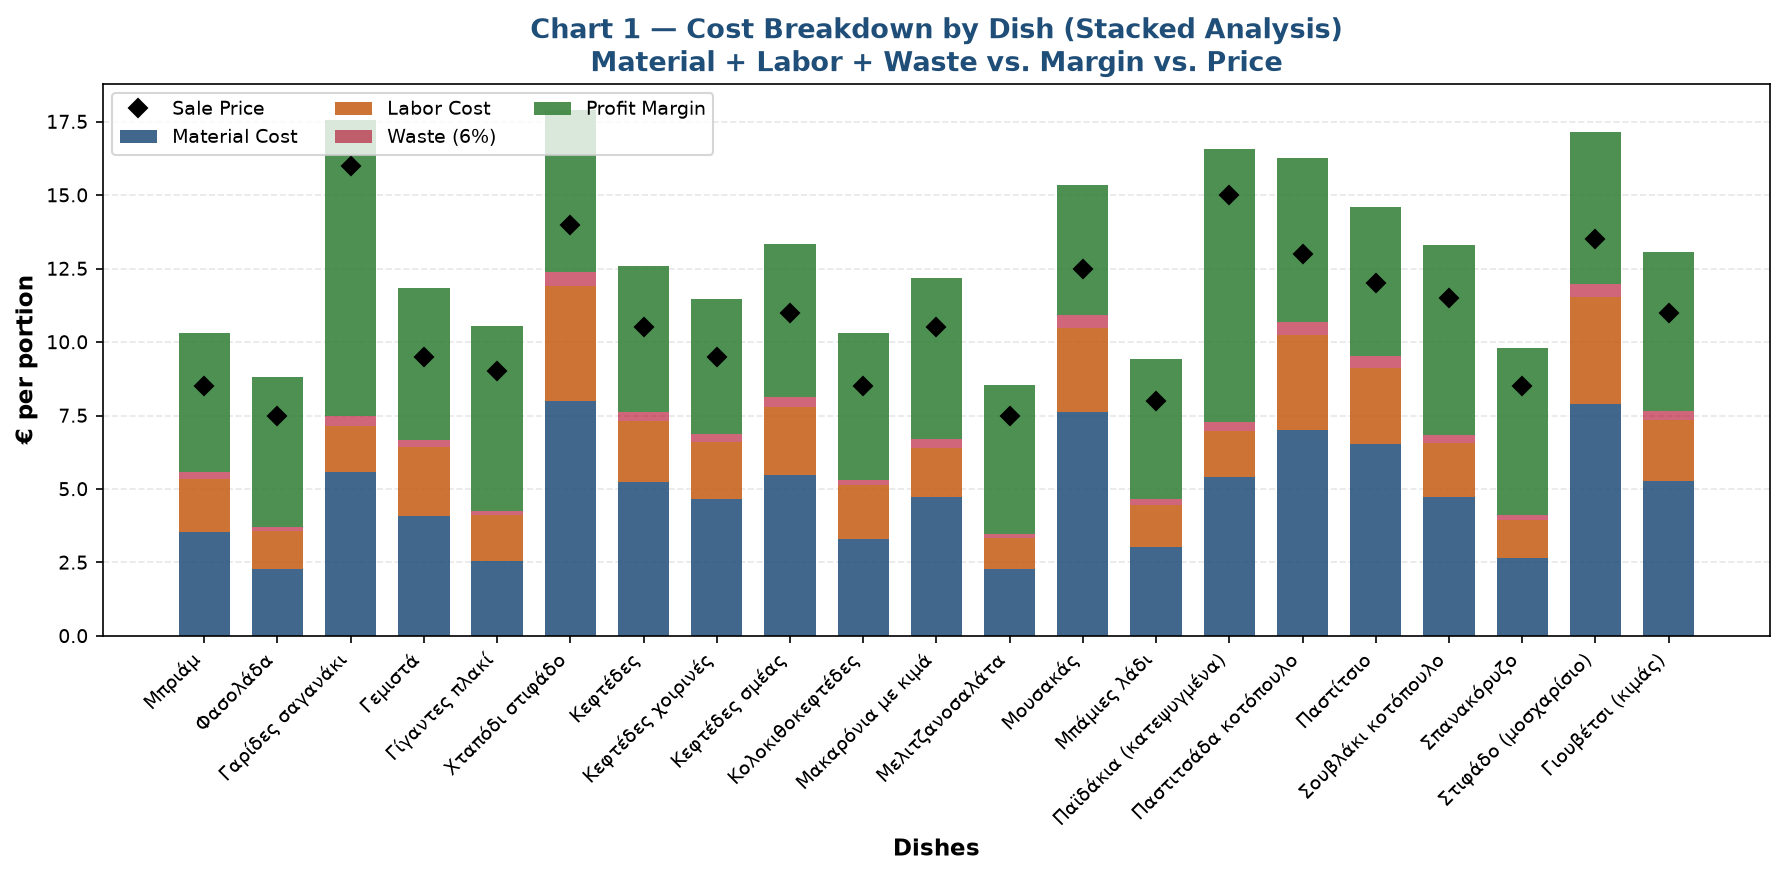
\includegraphics[width=\textwidth]{chart_01_cost_breakdown.png}
\caption{Αποδόμηση της τιμής πώλησης κάθε πιάτου σε κόστος υλικών, εργασίας,
σπατάλης και περιθώριο κέρδους. Οι μαύροι ρόμβοι σημειώνουν την τιμή πώλησης $P_d$.}
\label{fig:c1}
\end{figure}

\subsection{Κατάταξη αποδοτικότητας ανά εργατοώρα (Σχήμα~\ref{fig:c2})}
Το Σχήμα~\ref{fig:c2} ταξινομεί τα πιάτα κατά $\rho_d$ (περιθώριο ανά εργατοώρα).
Το πράσινο χρώμα σημειώνει τα πιάτα που επιλέγονται στη λύση του \en{LP}. Ο στενός
πόρος είναι ο χρόνος [περιορισμός~\eqref{eq:lplabor}]: όταν δύο πιάτα ανταγωνίζονται
για το ίδιο λεπτό κουζίνας, συμφέρει εκείνο που αποδίδει περισσότερο κέρδος \emph{ανά
λεπτό}. Η κατανομή των χρωμάτων επιβεβαιώνει ότι το πράσινο συγκεντρώνεται στην
κορυφή: το \en{LP} «γεμίζει» το μενού κατεβαίνοντας την κατάταξη μέχρι την εξάντληση
των 65 ωρών.

\begin{figure}[htbp]
\centering
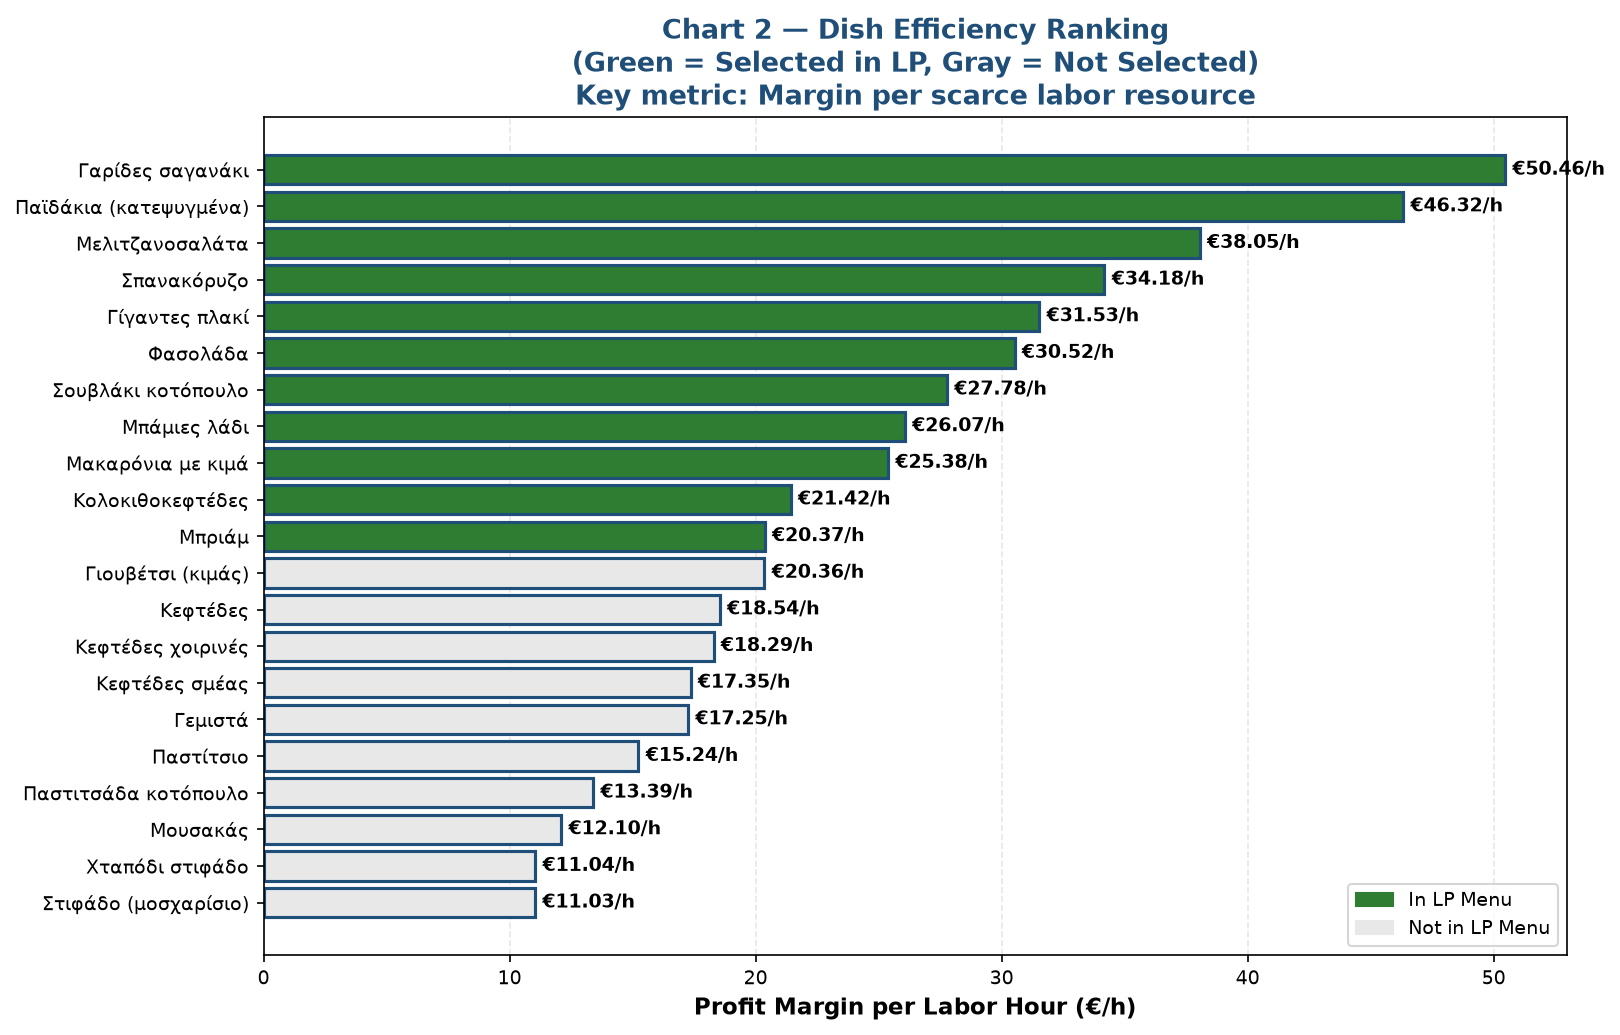
\includegraphics[width=0.92\textwidth]{chart_02_efficiency_ranking.png}
\caption{Κατάταξη των 21 πιάτων κατά περιθώριο ανά εργατοώρα $\rho_d$.
Πράσινο = επιλεγμένο στη λύση του \en{LP}, γκρι = μη επιλεγμένο.}
\label{fig:c2}
\end{figure}

\subsection{Σύγκριση \en{LP} και \en{MIP} (Σχήμα~\ref{fig:c3})}
Το Σχήμα~\ref{fig:c3} παραθέτει δίπλα-δίπλα τις παραγόμενες μερίδες $x_d$ στις δύο
λύσεις. Το \en{LP} κατανέμει συνολικά 332 μερίδες σε 11 πιάτα, ενώ το \en{MIP} 327
μερίδες σε 10 πιάτα. Το συνολικό μήνυμα είναι ότι το \en{MIP} \emph{συγκεντρώνει}
την παραγωγή σε λιγότερα πιάτα, ωθώντας τα στο όριο $D_d^{\max}$ ώστε να
αμορτίζονται καλύτερα τα πάγια κόστη.

\begin{figure}[htbp]
\centering
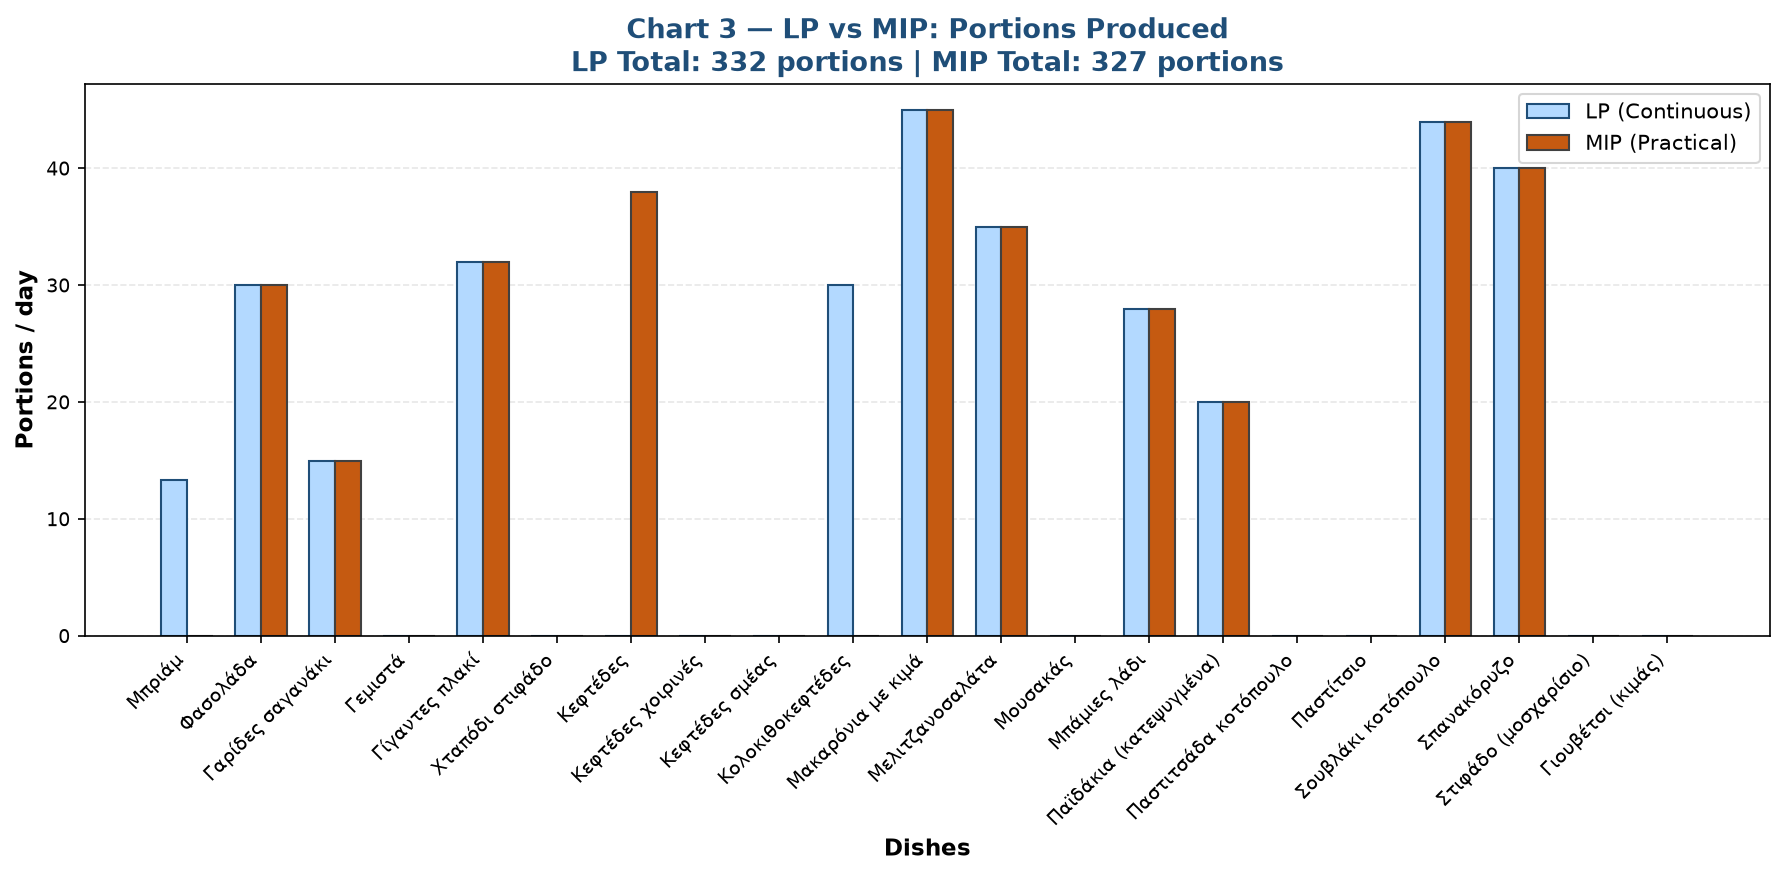
\includegraphics[width=\textwidth]{chart_03_portions_lp_vs_mip.png}
\caption{Μερίδες παραγωγής ανά πιάτο: \en{LP} (συνεχές, γαλάζιο) έναντι \en{MIP}
(πρακτικό, πορτοκαλί).}
\label{fig:c3}
\end{figure}

\subsection{Το βέλτιστο μενού του \en{MIP} (Σχήμα~\ref{fig:c4})}
Το \en{MIP} επιλέγει \textbf{ακριβώς 10 πιάτα}. Τονίζεται ότι το 10 \emph{δεν}
αποτελεί ανεξάρτητη ανακάλυψη του μοντέλου: είναι το άνω όριο $N_{\max}=10$ του
περιορισμού~\eqref{eq:mipsize}, το οποίο ενεργοποιείται. Το Σχήμα~\ref{fig:c4}
αναλύει τη συνεισφορά κάθε επιλεγμένου πιάτου (πράσινη μπάρα: μεικτή συνεισφορά
$m_d x_d$· κόκκινη: πάγιο κόστος $-f_d$· ετικέτα: καθαρή συνεισφορά).

\begin{figure}[htbp]
\centering
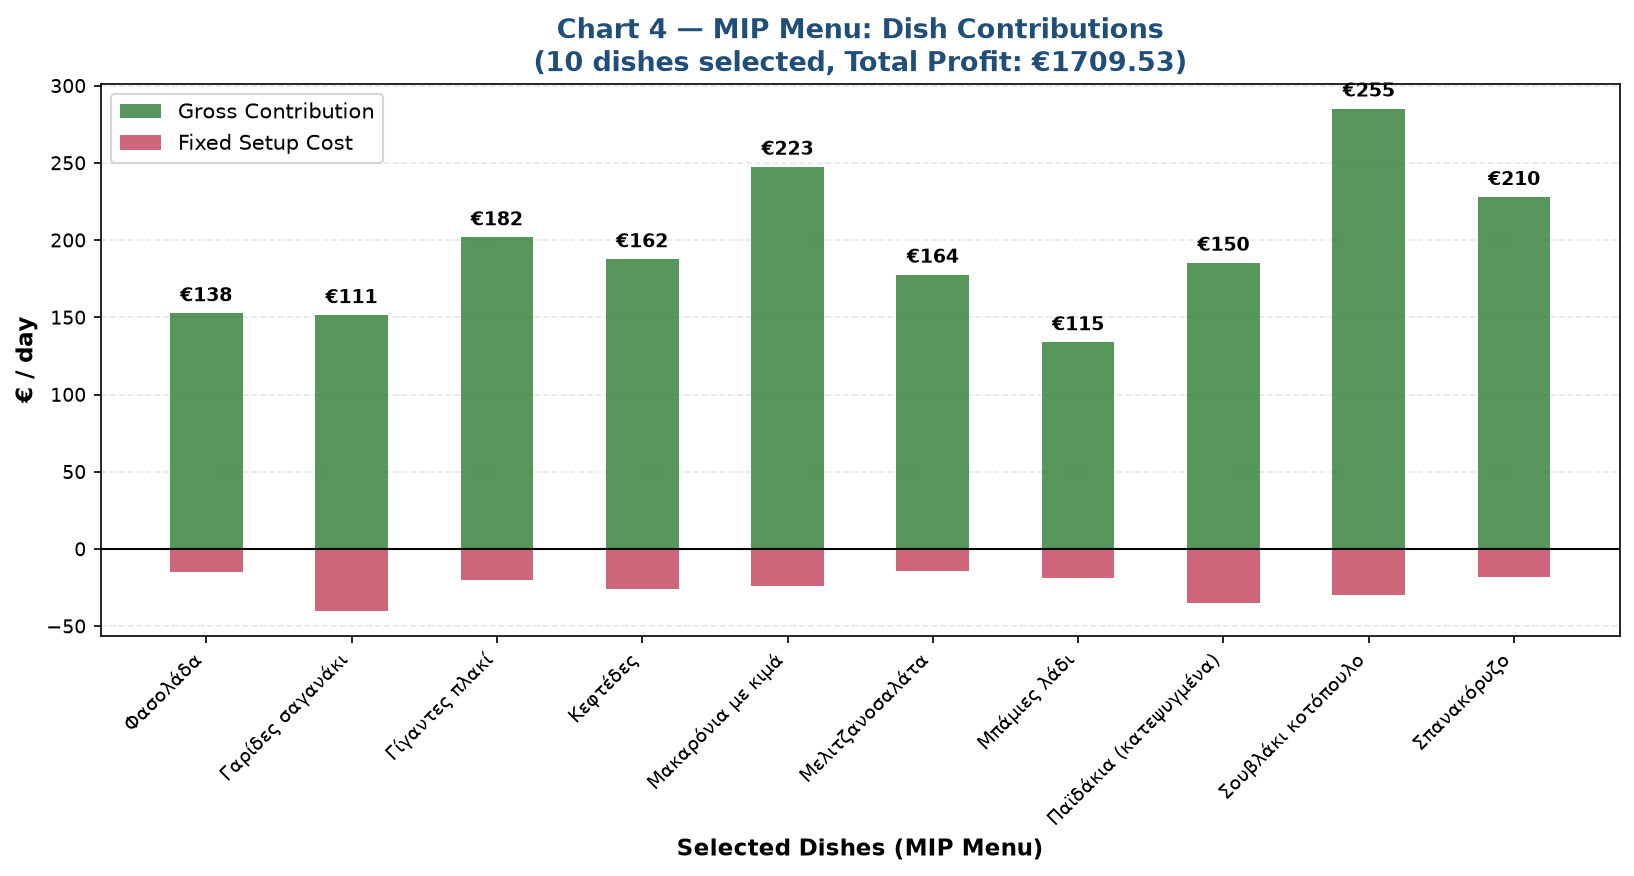
\includegraphics[width=0.95\textwidth]{chart_04_mip_contributions.png}
\caption{Καθαρή συνεισφορά κάθε επιλεγμένου πιάτου στο ημερήσιο κέρδος του \en{MIP}
(10 πιάτα, συνολικό κέρδος 1709,53\,€).}
\label{fig:c4}
\end{figure}

Το Σχήμα~\ref{fig:c5demand} επιβεβαιώνει ότι η λύση σέβεται τα όρια της αγοράς
[περιορισμοί~\eqref{eq:miplink}--\eqref{eq:mipmin}]: η παραγωγή κάθε πιάτου βρίσκεται
πάντα μεταξύ της ελάχιστης και της μέγιστης ζήτησης, και για τα πιο αποδοτικά πιάτα
«κολλάει» στη μέγιστη ζήτηση.

\begin{figure}[htbp]
\centering
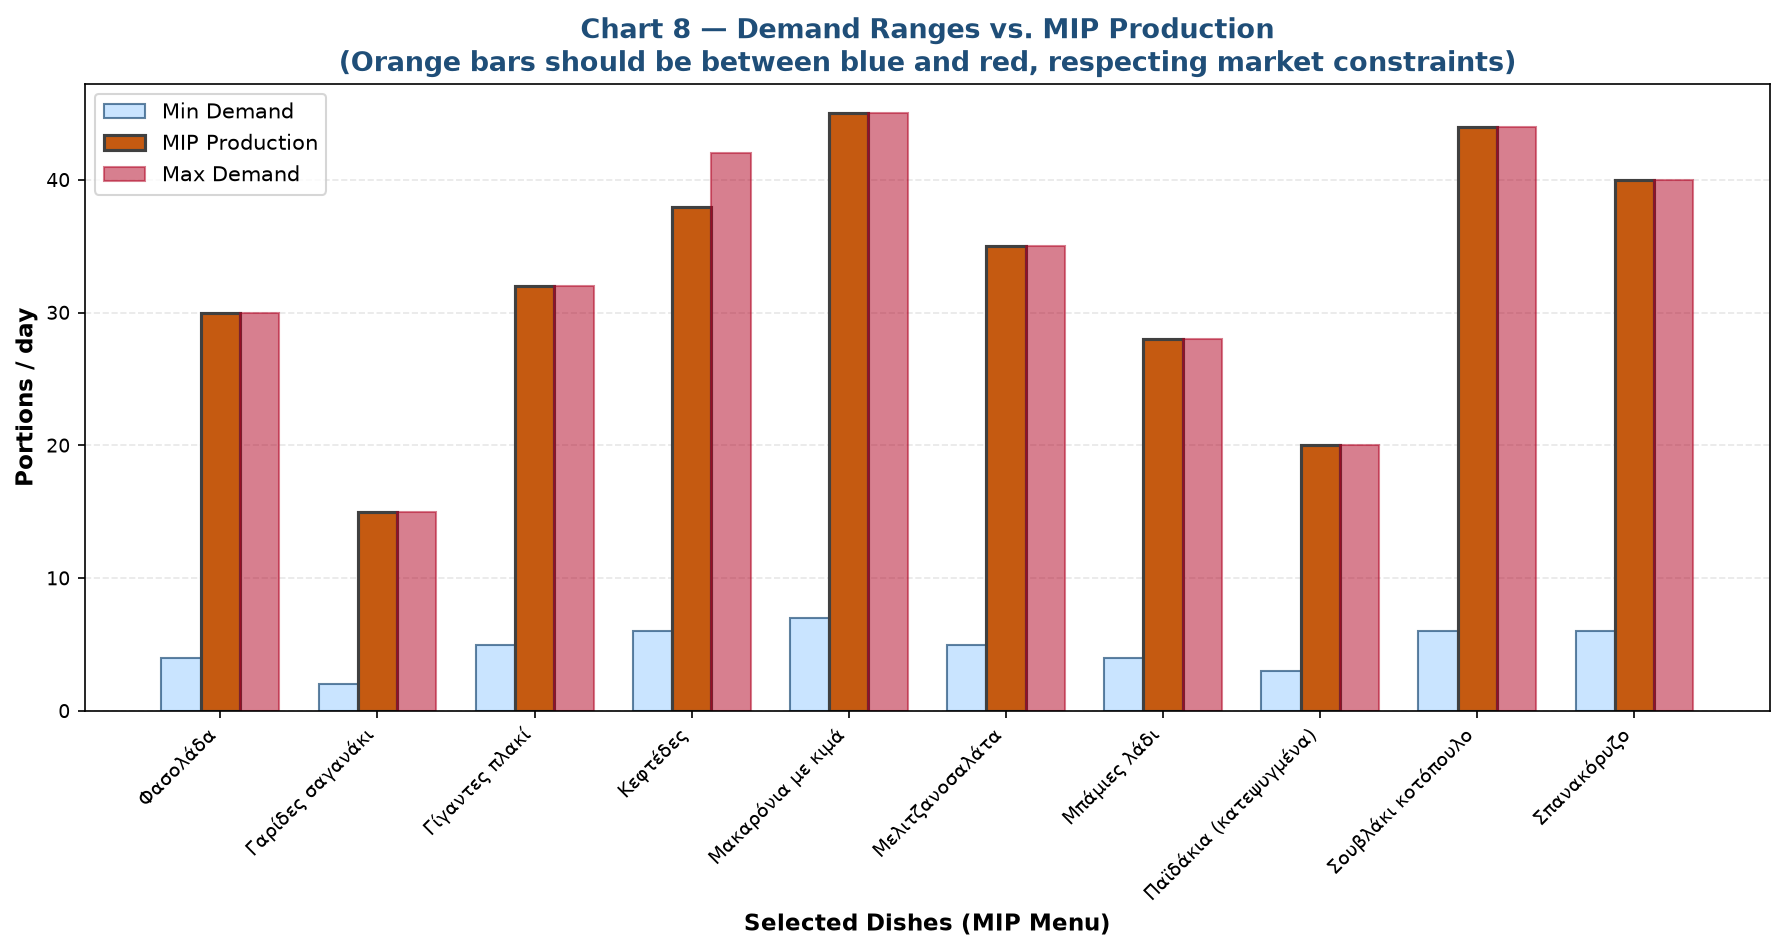
\includegraphics[width=\textwidth]{chart_08_demand_vs_production.png}
\caption{Ελάχιστη ζήτηση (γαλάζιο), παραγωγή \en{MIP} (πορτοκαλί) και μέγιστη ζήτηση
(κόκκινο) ανά επιλεγμένο πιάτο. Η παραγωγή βρίσκεται πάντα εντός των ορίων της αγοράς.}
\label{fig:c5demand}
\end{figure}

% =====================================================================
\section{Δυϊκότητα και Οικονομική Ερμηνεία}\label{sec:duality}
Η ενότητα αυτή εμβαθύνει στη θεωρία του Γραμμικού Προγραμματισμού, αντλώντας από τη
βέλτιστη λύση του \en{LP} την πλήρη \emph{δυϊκή} της πληροφορία (αρχείο
\en{duality.py}). Η δυϊκότητα δεν είναι απλώς μαθηματική κομψότητα: μετατρέπει τις
ποιοτικές παρατηρήσεις των προηγούμενων ενοτήτων («ο χρόνος είναι ο στενός πόρος»,
«ο Μουσακάς αποκλείεται λόγω κόστους ευκαιρίας») σε \emph{αυστηρά, μετρήσιμα} μεγέθη.

\subsection{Το δυϊκό πρόβλημα}
Σε κάθε περιορισμό του πρωτεύοντος αντιστοιχεί μια \emph{δυϊκή μεταβλητή} (σκιώδης
τιμή): στον περιορισμό εργασίας~\eqref{eq:lplabor} η μεταβλητή $u\ge 0$, και σε
κάθε περιορισμό ζήτησης~\eqref{eq:lpdemand} μια μεταβλητή $v_d\ge 0$. Το δυϊκό του
πρωτεύοντος \en{LP} [\eqref{eq:lpobj}--\eqref{eq:lpdemand}] είναι:
\begin{align}
\min\; W &= H\,u + \sum_{d\in D} D_d^{\max}\, v_d \label{eq:dualobj}\\
\text{υπό:}\quad \tfrac{t_d}{60}\,u + v_d &\ge m_d && \forall d\in D \label{eq:dualcon}\\
u \ge 0,\; v_d &\ge 0 && \forall d\in D. \nonumber
\end{align}
Υπάρχει ένας δυϊκός περιορισμός~\eqref{eq:dualcon} ανά πρωτεύουσα μεταβλητή $x_d$.
Η οικονομική του ανάγνωση είναι διαφωτιστική: το αριστερό μέλος είναι το
\emph{αποτιμημένο κόστος ευκαιρίας} μιας μερίδας του $d$ — η αξία των πόρων (χρόνος
$\tfrac{t_d}{60}u$ και «δικαίωμα ζήτησης» $v_d$) που καταναλώνει. Ο περιορισμός
απαιτεί αυτό να μην είναι μικρότερο από το περιθώριο $m_d$ που αποδίδει το πιάτο.

\subsection{Ισχυρή δυϊκότητα}
Επιλύοντας \emph{ανεξάρτητα} το πρωτεύον και το δυϊκό με τον \en{CBC}, οι δύο
βέλτιστες τιμές ταυτίζονται:
\[
Z^\star_{\mathrm{LP}} = W^\star = \LPobj\;€/\text{ημέρα},\qquad
|Z^\star - W^\star| < 10^{-3}.
\]
Αυτή είναι ακριβώς η πρόβλεψη του \emph{Θεωρήματος Ισχυρής Δυϊκότητας}~\cite{bertsimas}:
για ένα εφικτό και φραγμένο \en{LP}, το πρωτεύον και το δυϊκό έχουν την ίδια βέλτιστη
τιμή. Η αριθμητική επιβεβαίωση λειτουργεί και ως έλεγχος ορθότητας ολόκληρου του μοντέλου.

\subsection{Σκιώδεις τιμές (\en{shadow prices})}
Η βέλτιστη δυϊκή λύση δίνει τη \textbf{σκιώδη τιμή της εργασίας}
\[
u^\star = \LaborShadow\;€/\text{ώρα}.
\]
Ερμηνεία: μία επιπλέον διαθέσιμη εργατοώρα θα αύξανε το βέλτιστο μεικτό κέρδος του
\en{LP} κατά $\LaborShadow$\,€. Καθώς το ωρομίσθιο είναι μόλις $w=\LaborWage$\,€/ώρα,
\emph{κάθε επιπλέον ώρα εργασίας αποδίδει καθαρό όφελος} $u^\star - w \approx 12{,}6$\,€.
Αυτό αποτελεί ισχυρότατο, ποσοτικό επιχείρημα υπέρ της πρόσληψης προσωπικού.

\paragraph{Συμφιλίωση με την ανάλυση ευαισθησίας.} Στην Ενότητα~\ref{sec:sensitivity}
(Πίνακας~\ref{tab:labor}) το \emph{οριακό όφελος} της εργασίας στο \en{MIP}, όπως
προκύπτει από πεπερασμένες διαφορές γύρω από τις 65 ώρες, είναι $\approx 14{,}8$\,€/ώρα
— μικρότερο από τη σκιώδη τιμή $u^\star=\LaborShadow$\,€/ώρα του \en{LP}. Η διαφορά
είναι \emph{αναμενόμενη} και διδακτική: (i)~το \en{LP} αγνοεί τα πάγια κόστη, οπότε
η πλήρης αξία μιας ώρας εμφανίζεται ακέραιη· (ii)~στο \en{MIP} μέρος της επιπλέον
ώρας «ξοδεύεται» στην ενεργοποίηση/στήριξη πιάτων με πάγιο κόστος, μειώνοντας το
καθαρό οριακό όφελος. Και τα δύο νούμερα, πάντως, υπερβαίνουν κατά πολύ το ωρομίσθιο.

\subsection{Μειωμένο κόστος: γιατί αποκλείονται πιάτα}
Για κάθε πιάτο ορίζεται το \emph{μειωμένο κόστος}
\begin{equation}
r_d = m_d - \Big(\tfrac{t_d}{60}\,u^\star + v_d^\star\Big).
\label{eq:reduced}
\end{equation}
Για ένα πιάτο που \emph{δεν} παράγεται ισχύει $r_d \le 0$: το $|r_d|$ είναι το
\textbf{κόστος ευκαιρίας} — πόσο θα \emph{μειωνόταν} το ημερήσιο κέρδος αν
επιβάλλαμε την παραγωγή μίας μερίδας του $d$. Ο Πίνακας~\ref{tab:duality} παραθέτει
τα μεγέθη αυτά για όλα τα πιάτα (η αριθμητική ταύτιση της σχέσης~\eqref{eq:reduced}
με τα $r_d$ που επιστρέφει ο επιλύτης επαληθεύτηκε με σφάλμα $0$).

Το αποτέλεσμα-κλειδί: για τα πιάτα που παράγονται στο όριο της ζήτησής τους, το
$v_d^\star>0$· για όσα παράγονται ελεύθερα, $r_d=0$· και για τα αποκλειόμενα, το
$r_d<0$ ποσοτικοποιεί \emph{ακριβώς} την αιτία του αποκλεισμού. Ο Μουσακάς, για
παράδειγμα, έχει $r=-3{,}03$\,€: αν και κερδοφόρος ($m=4{,}44$\,€), το κόστος
ευκαιρίας του χρόνου του, $\tfrac{22}{60}\cdot\LaborShadow = 7{,}47$\,€, υπερβαίνει
το περιθώριό του κατά ακριβώς $3{,}03$\,€. Το Σχήμα~\ref{fig:c9} αποτυπώνει αυτή τη
σύγκριση οπτικά για όλα τα αποκλειόμενα πιάτα.

\begin{table}[htbp]
\centering
\caption{Δυϊκή ανάλυση των 21 πιάτων. $m$: περιθώριο (€/μερίδα)· $t$: λεπτά εργασίας·
$x^\star$: μερίδες στη λύση \en{LP}· $r$: μειωμένο κόστος (€/μερίδα)· $v$: σκιώδης
τιμή ζήτησης (€/μερίδα). Πάνω: παραγόμενα (ταξ.\ κατά $v$)· κάτω: αποκλειόμενα
(ταξ.\ κατά $r$).}
\label{tab:duality}
\small
\setlength{\tabcolsep}{6pt}
\begin{tabular}{@{}lrrrrrl@{}}
\toprule
\textbf{Πιάτο} & $m$ & $t$ & $x^\star$ & $r$ & $v$ & \textbf{Κατάσταση} \\
\midrule
Γαρίδες σαγανάκι & 10,09 & 12 & 15,0 & 0,00 & 6,02 & παράγεται \\
Παϊδάκια (κατεψυγμένα) & 9,26 & 12 & 20,0 & 0,00 & 5,19 & παράγεται \\
Μελιτζανοσαλάτα & 5,07 & 8 & 35,0 & 0,00 & 2,36 & παράγεται \\
Σπανακόρυζο & 5,70 & 10 & 40,0 & 0,00 & 2,30 & παράγεται \\
Γίγαντες πλακί & 6,31 & 12 & 32,0 & 0,00 & 2,23 & παράγεται \\
Σουβλάκι κοτόπουλο & 6,48 & 14 & 44,0 & 0,00 & 1,73 & παράγεται \\
Φασολάδα & 5,09 & 10 & 30,0 & 0,00 & 1,69 & παράγεται \\
Μακαρόνια με κιμά & 5,50 & 13 & 45,0 & 0,00 & 1,09 & παράγεται \\
Μπάμιες λάδι & 4,78 & 11 & 28,0 & 0,00 & 1,04 & παράγεται \\
Κολοκιθοκεφτέδες & 5,00 & 14 & 30,0 & 0,00 & 0,25 & παράγεται \\
Μπριάμ & 4,75 & 14 & 13,4 & 0,00 & 0,00 & παράγεται \\
\addlinespace
Χταπόδι στιφάδο & 5,52 & 30 & 0,0 & -4,66 & 0,00 & αποκλείεται \\
Στιφάδο (μοσχαρίσιο) & 5,15 & 28 & 0,0 & -4,36 & 0,00 & αποκλείεται \\
Μουσακάς & 4,44 & 22 & 0,0 & -3,03 & 0,00 & αποκλείεται \\
Παστιτσάδα κοτόπουλο & 5,58 & 25 & 0,0 & -2,91 & 0,00 & αποκλείεται \\
Παστίτσιο & 5,08 & 20 & 0,0 & -1,71 & 0,00 & αποκλείεται \\
Γεμιστά & 5,18 & 18 & 0,0 & -0,94 & 0,00 & αποκλείεται \\
Κεφτέδες σμέας & 5,21 & 18 & 0,0 & -0,91 & 0,00 & αποκλείεται \\
Κεφτέδες χοιρινές & 4,57 & 15 & 0,0 & -0,52 & 0,00 & αποκλείεται \\
Κεφτέδες & 4,94 & 16 & 0,0 & -0,49 & 0,00 & αποκλείεται \\
Γιουβέτσι (κιμάς) & 5,43 & 16 & 0,0 & 0,00 & 0,00 & αποκλείεται \\
\bottomrule
\end{tabular}

\end{table}

\begin{figure}[htbp]
\centering
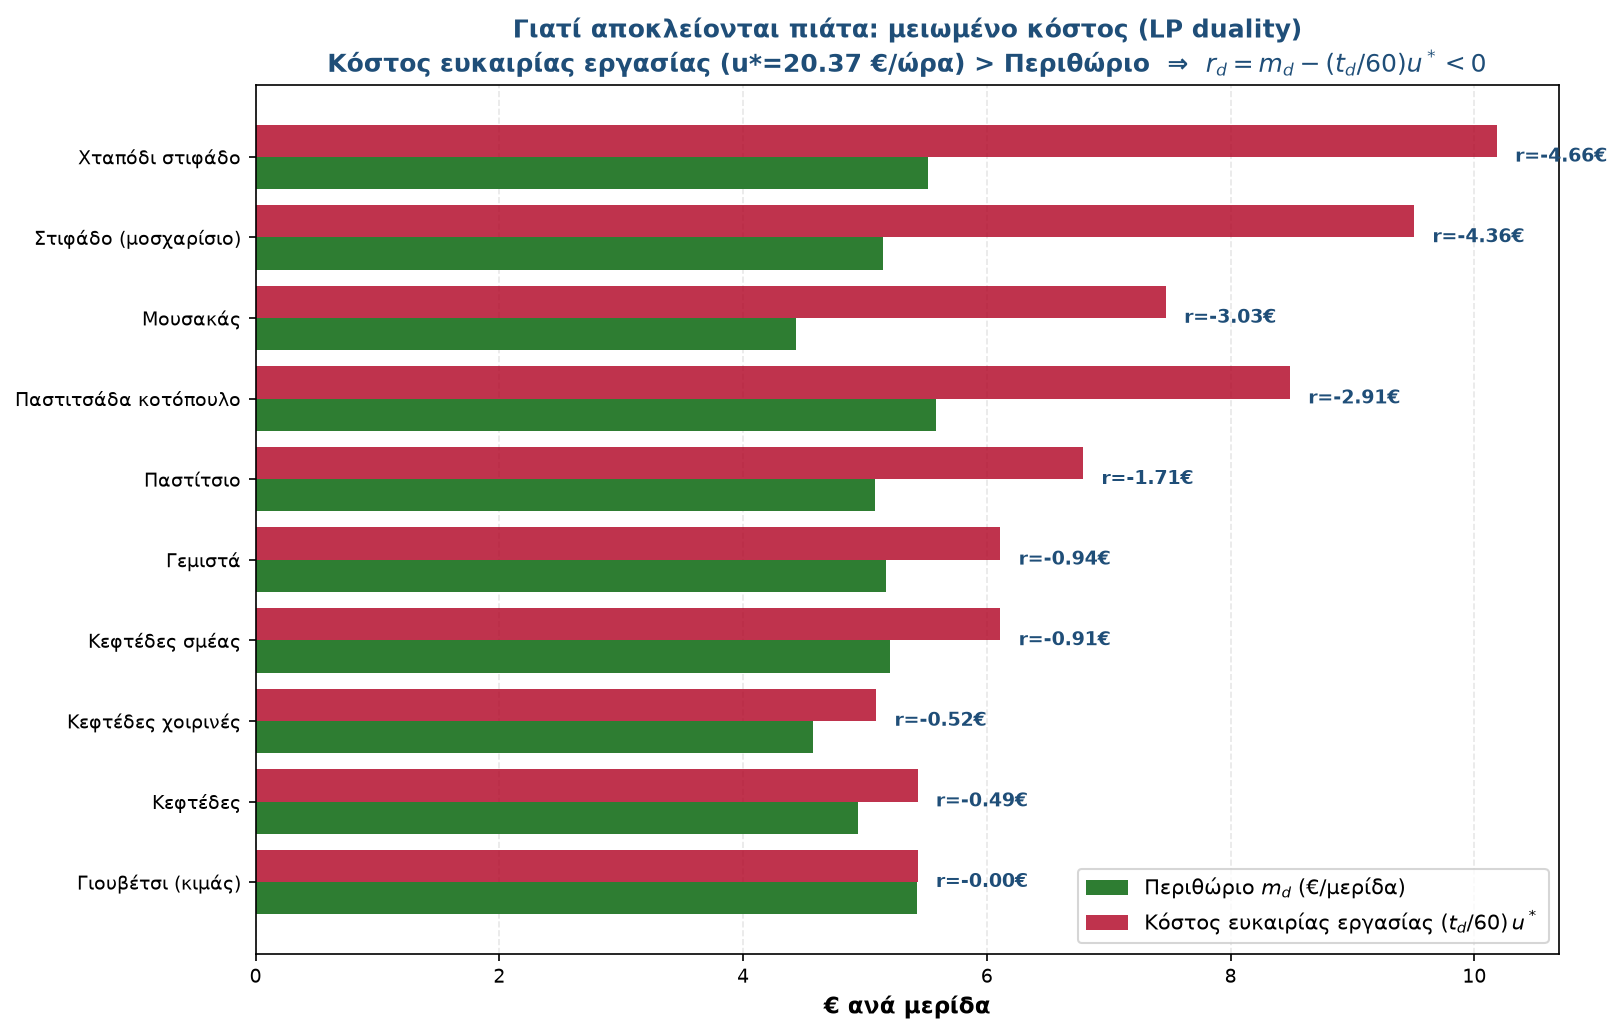
\includegraphics[width=0.92\textwidth]{chart_09_reduced_cost.png}
\caption{Ανάλυση μειωμένου κόστους των αποκλειόμενων πιάτων. Για κάθε πιάτο το
κόστος ευκαιρίας εργασίας $(t_d/60)\,u^\star$ (κόκκινο) υπερβαίνει το περιθώριο
$m_d$ (πράσινο)· η διαφορά είναι το (αρνητικό) μειωμένο κόστος $r_d$.}
\label{fig:c9}
\end{figure}

\subsection{Συμπληρωματική χαλαρότητα}
Η βέλτιστη λύση επαληθεύει πλήρως τις συνθήκες \emph{συμπληρωματικής χαλαρότητας}
(\en{complementary slackness}), που συνδέουν πρωτεύον και δυϊκό:
\begin{align}
u^\star\cdot\Big(H - \textstyle\sum_d \tfrac{t_d}{60}x_d^\star\Big) &= 0
   &&\text{(εργασία)}\\
v_d^\star\cdot\big(D_d^{\max} - x_d^\star\big) &= 0 &&\forall d \quad\text{(ζήτηση)}\\
x_d^\star\cdot r_d &= 0 &&\forall d \quad\text{(μεταβλητές)}
\end{align}
Πρακτικά: αφού $u^\star>0$, ο περιορισμός εργασίας είναι \emph{δεσμευτικός} (οι 65
ώρες εξαντλούνται πλήρως)· ένα πιάτο έχει θετική σκιώδη τιμή ζήτησης $v_d^\star>0$
\emph{μόνο} αν παράγεται στο όριό του $D_d^{\max}$· και ένα πιάτο έχει μη μηδενικό
μειωμένο κόστος \emph{μόνο} αν δεν παράγεται. Οι σχέσεις αυτές ικανοποιούνται
αριθμητικά για κάθε πιάτο, κλείνοντας συνεπώς τον κύκλο πρωτεύον--δυϊκό.

\subsection{Οριακή αξία ζήτησης (Σχήμα~\ref{fig:c10})}
Οι σκιώδεις τιμές ζήτησης $v_d^\star$ έχουν άμεση διαχειριστική χρήση: δείχνουν πού
αποδίδει περισσότερο μία επένδυση σε διαφήμιση/\en{marketing}. Το Σχήμα~\ref{fig:c10}
τις κατατάσσει· οι Γαρίδες σαγανάκι ($v=6{,}02$\,€/μερίδα) και τα Παϊδάκια
($v=5{,}19$\,€/μερίδα) είναι εκείνα για τα οποία μία επιπλέον μονάδα ζήτησης θα
απέδιδε το μεγαλύτερο επιπλέον κέρδος — ακριβώς επειδή παράγονται ήδη στο όριο της
αγοράς τους και είναι εξαιρετικά αποδοτικά ανά ώρα.

\begin{figure}[htbp]
\centering
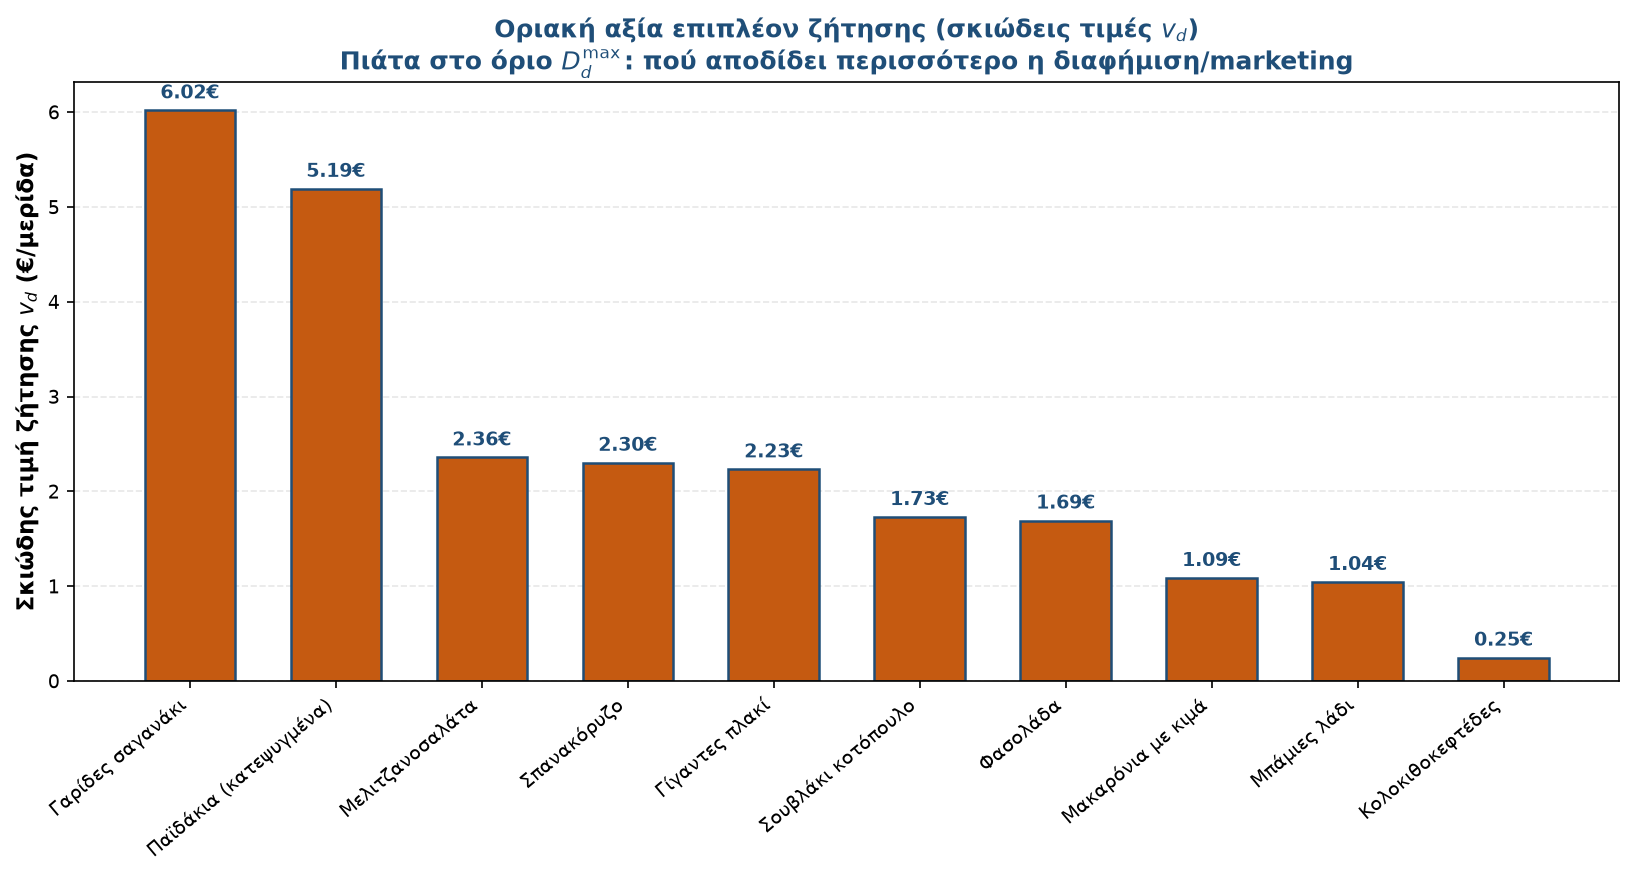
\includegraphics[width=0.92\textwidth]{chart_10_demand_shadow.png}
\caption{Σκιώδεις τιμές ζήτησης $v_d^\star$ για τα πιάτα που παράγονται στο όριο
$D_d^{\max}$: οριακή αξία μίας επιπλέον μονάδας ζήτησης (προτεραιότητα \en{marketing}).}
\label{fig:c10}
\end{figure}

% =====================================================================
\section{Παραμετρική Ανάλυση και Εύρος Ευστάθειας}\label{sec:ranging}
Η δυϊκή λύση δίνει τις σκιώδεις τιμές \emph{στο τρέχον σημείο}. Ένα φυσικό επόμενο
ερώτημα της θεωρίας~\cite{bertsimas,winston} είναι: \emph{για πόσο} παραμένουν αυτές
έγκυρες; Η \emph{ανάλυση εύρους} (\en{ranging}) απαντά σε δύο εκδοχές: μεταβολή του
δεξιού μέλους ενός περιορισμού, και μεταβολή ενός συντελεστή της αντικειμενικής.

\subsection{Εύρος δεξιού μέλους: οι εργατοώρες (Σχήμα~\ref{fig:c11})}
Καθώς μεταβάλλονται οι διαθέσιμες ώρες $H$, το βέλτιστο κέρδος του \en{LP} είναι
\emph{τμηματικά γραμμικό} και κοίλο: κάθε ευθύγραμμο τμήμα αντιστοιχεί σε μια
βέλτιστη βάση, και η κλίση του είναι ακριβώς η σκιώδης τιμή $u^\star$. Η τρέχουσα
σκιώδης τιμή $u^\star=\LaborShadow$\,€/ώρα παραμένει σταθερή όσο δεν αλλάζει η βάση:
\[
H \in [\,\Hlow,\ \Hhigh\,]\ \text{ώρες}\qquad
(\text{επιτρεπτή μείωση } \Hdec,\ \text{επιτρεπτή αύξηση } \Hinc\ \text{ώρες}).
\]
Εντός αυτού του εύρους, κάθε επιπλέον ώρα αξίζει σταθερά $\LaborShadow$\,€. Πέρα από
τα όρια, η βάση αλλάζει (κάποιο πιάτο φτάνει το όριο ζήτησής του ή εξαντλείται) και η
οριακή αξία της εργασίας \emph{μειώνεται} — γι' αυτό η καμπύλη του
Σχήματος~\ref{fig:c11} «λυγίζει» σε φθίνουσες κλίσεις.

\begin{figure}[htbp]
\centering
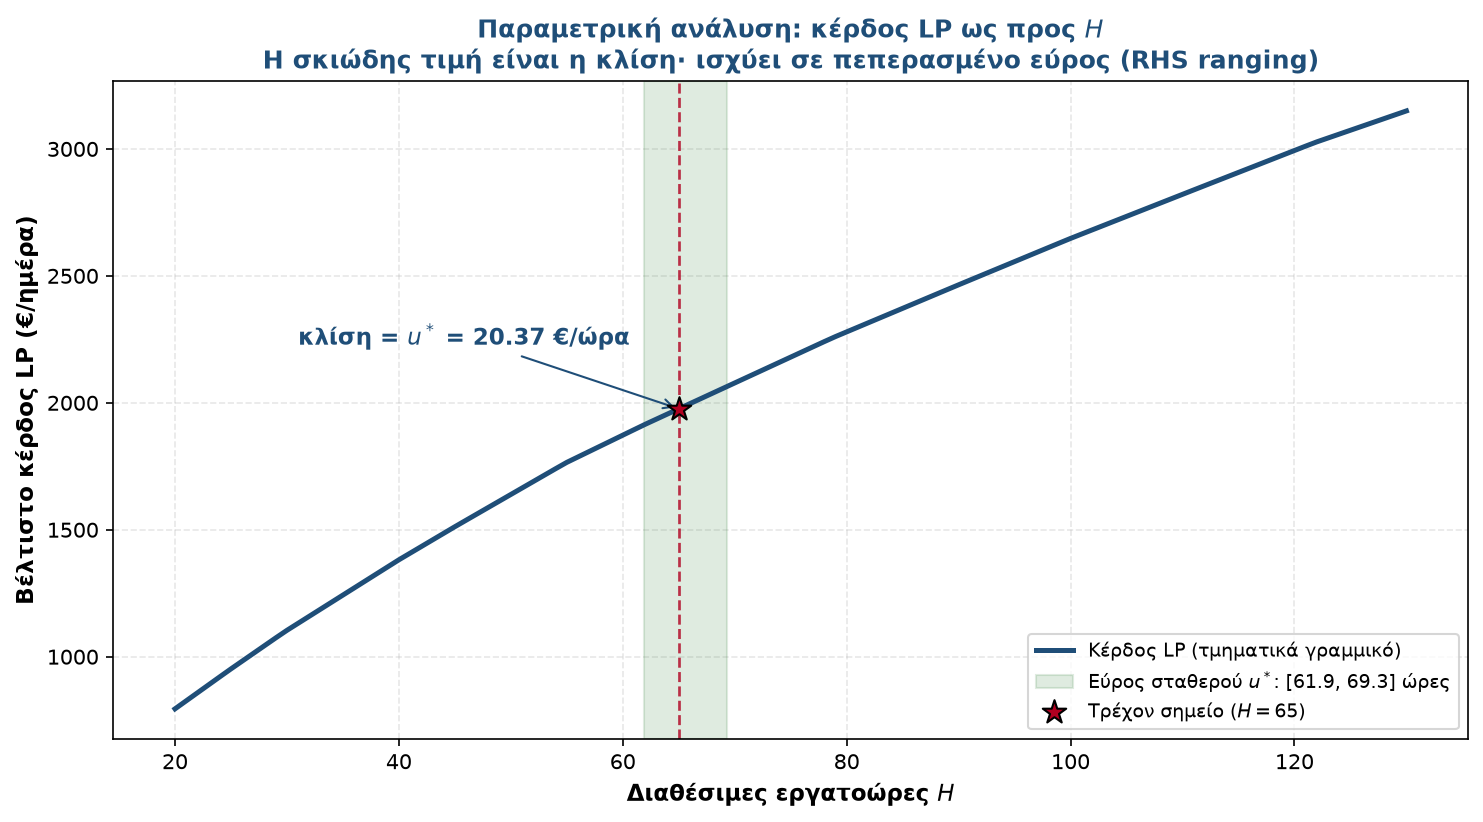
\includegraphics[width=0.82\textwidth]{chart_11_parametric_labor.png}
\caption{Παραμετρική ανάλυση: βέλτιστο κέρδος \en{LP} ως συνάρτηση των εργατοωρών
$H$. Η σκιώδης τιμή είναι η κλίση της (τμηματικά γραμμικής) καμπύλης· ισχύει στο
πράσινο εύρος $[\Hlow, \Hhigh]$.}
\label{fig:c11}
\end{figure}

\subsection{Εύρος συντελεστών της αντικειμενικής: τα περιθώρια}
Το δεύτερο ερώτημα είναι πόσο μπορεί να μεταβληθεί το περιθώριο $m_d$ ενός πιάτου
\emph{χωρίς} να αλλάξει η βέλτιστη λύση $x^\star$. Ο Πίνακας~\ref{tab:ranging}
δίνει την επιτρεπτή αύξηση και μείωση για κάθε πιάτο. Δύο διακριτές συμπεριφορές:
\begin{itemize}
  \item \textbf{Παραγόμενα πιάτα:} το περιθώριο μπορεί να \emph{αυξηθεί} απεριόριστα
  (παραμένουν στο μενού)· η επιτρεπτή \emph{μείωση} δείχνει πόση πτώση αντέχουν πριν
  εγκαταλείψουν τη λύση (π.χ.\ οι Γαρίδες αντέχουν πτώση $6{,}02$\,€).
  \item \textbf{Αποκλειόμενα πιάτα:} συμμετρικά, η επιτρεπτή \emph{αύξηση} ισούται
  \textbf{ακριβώς με το $|$μειωμένο κόστος$|$} της Ενότητας~\ref{sec:duality} —
  πόσο πρέπει να ανέβει το περιθώριο για να «μπει» το πιάτο. Για τον Μουσακά:
  αύξηση $3{,}03$\,€, δηλαδή ακριβώς το $|r_{\text{μουσ.}}|$. Αυτή η ταύτιση είναι
  θεωρητικά αναμενόμενη και επιβεβαιώνει τη συνέπεια δυϊκότητας--ranging.
\end{itemize}

\begin{table}[htbp]
\centering
\caption{Εύρος συντελεστών της αντικειμενικής: επιτρεπτή μεταβολή του περιθωρίου
$m_d$ (€/μερίδα) που διατηρεί αμετάβλητη τη βέλτιστη λύση $x^\star$ του \en{LP}.
Για τα αποκλειόμενα πιάτα, η επιτρεπτή αύξηση $=|r_d|$ (μειωμένο κόστος).}
\label{tab:ranging}
\small
\setlength{\tabcolsep}{6pt}
\begin{tabular}{@{}lrlrr@{}}
\toprule
\textbf{Πιάτο} & $m$ & \textbf{Κατάσταση} & \textbf{Επιτρ. αύξηση} & \textbf{Επιτρ. μείωση} \\
\midrule
Γαρίδες σαγανάκι & 10,09 & παράγεται & $\infty$ & 6,02 \\
Παϊδάκια (κατεψυγμένα) & 9,26 & παράγεται & $\infty$ & 5,19 \\
Σουβλάκι κοτόπουλο & 6,48 & παράγεται & $\infty$ & 1,73 \\
Γίγαντες πλακί & 6,31 & παράγεται & $\infty$ & 2,23 \\
Σπανακόρυζο & 5,70 & παράγεται & $\infty$ & 2,30 \\
Μακαρόνια με κιμά & 5,50 & παράγεται & $\infty$ & 1,09 \\
Φασολάδα & 5,09 & παράγεται & $\infty$ & 1,69 \\
Μελιτζανοσαλάτα & 5,07 & παράγεται & $\infty$ & 2,36 \\
Κολοκιθοκεφτέδες & 5,00 & παράγεται & $\infty$ & 0,25 \\
Μπάμιες λάδι & 4,78 & παράγεται & $\infty$ & 1,04 \\
Μπριάμ & 4,75 & παράγεται & 0,25 & 0,00 \\
\addlinespace
Χταπόδι στιφάδο & 5,52 & αποκλείεται & 4,66 & $\infty$ \\
Στιφάδο (μοσχαρίσιο) & 5,15 & αποκλείεται & 4,36 & $\infty$ \\
Μουσακάς & 4,44 & αποκλείεται & 3,03 & $\infty$ \\
Παστιτσάδα κοτόπουλο & 5,58 & αποκλείεται & 2,91 & $\infty$ \\
Παστίτσιο & 5,08 & αποκλείεται & 1,71 & $\infty$ \\
Γεμιστά & 5,18 & αποκλείεται & 0,93 & $\infty$ \\
Κεφτέδες σμέας & 5,21 & αποκλείεται & 0,90 & $\infty$ \\
Κεφτέδες χοιρινές & 4,57 & αποκλείεται & 0,52 & $\infty$ \\
Κεφτέδες & 4,94 & αποκλείεται & 0,49 & $\infty$ \\
Γιουβέτσι (κιμάς) & 5,43 & αποκλείεται & 0,00 & $\infty$ \\
\bottomrule
\end{tabular}

\end{table}

% =====================================================================
\section{Ανάλυση Ευαισθησίας}\label{sec:sensitivity}
Στην ανάλυση ευαισθησίας μεταβάλλεται μία παράμετρος κάθε φορά και το \en{MIP}
επιλύεται εκ νέου, ώστε να αποτιμηθεί πόσο «εύθραυστη» ή «εύρωστη» είναι η βέλτιστη
λύση.

\subsection{Κόστος πρώτων υλών (Σχήμα~\ref{fig:c6})}
Όλες οι τιμές υλικών πολλαπλασιάζονται ομοιόμορφα με συντελεστή από 0,75 έως 1,50.
Το κέρδος μεταβάλλεται σχεδόν γραμμικά (Σχήμα~\ref{fig:c6}): μια γενικευμένη
ανατίμηση 25\% «κοστίζει» περίπου 198\,€/ημέρα. Το κόστος υλικών είναι ο παράγοντας
με τη μεγαλύτερη επίδραση, άρα η διαπραγμάτευση με προμηθευτές έχει άμεσο αποτύπωμα
στην κερδοφορία.

\begin{figure}[htbp]
\centering
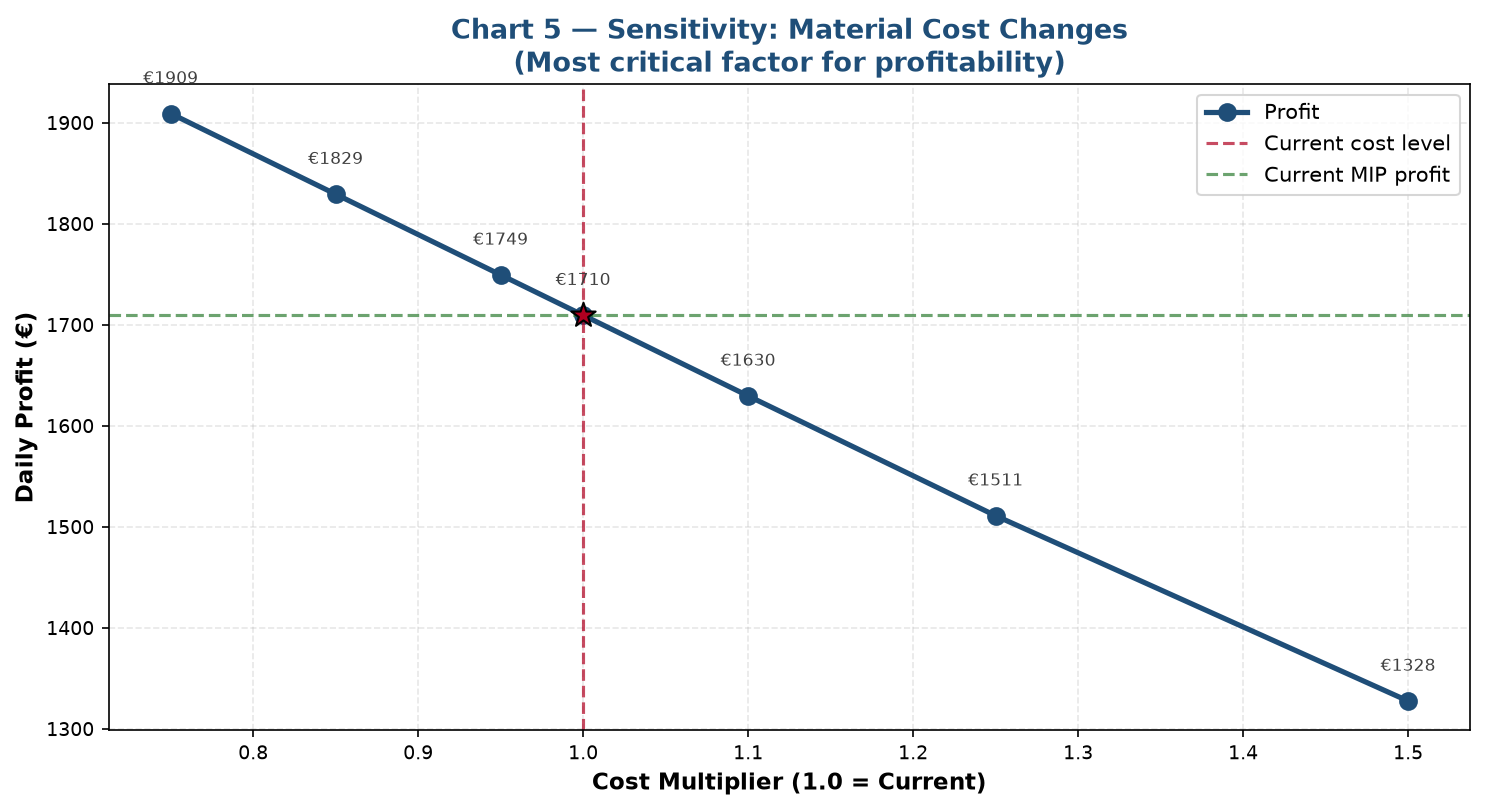
\includegraphics[width=0.78\textwidth]{chart_05_sensitivity_cost.png}
\caption{Ευαισθησία του ημερήσιου κέρδους σε ομοιόμορφη μεταβολή του κόστους υλικών.
Το αστέρι σημειώνει το τρέχον επίπεδο ($\times 1{,}0$).}
\label{fig:c6}
\end{figure}

\begin{table}[htbp]
\centering
\begin{minipage}{0.48\textwidth}
\centering
\caption{Ευαισθησία στο κόστος υλικών (\en{MIP}).}
\label{tab:material}
\small
\begin{tabular}{@{}lrr@{}}
\toprule
\textbf{Πολ/στής} & \textbf{Κέρδος (€)} & \textbf{Πιάτα} \\
\midrule
$\times$0,75 & 1909,24 & 10 \\
$\times$0,85 & 1829,36 & 10 \\
$\times$0,95 & 1749,47 & 10 \\
\bfseries $\times$1,00 & \bfseries 1709,53 & \bfseries 10 \\
$\times$1,05 & 1669,59 & 10 \\
$\times$1,15 & 1589,71 & 10 \\
$\times$1,25 & 1511,05 & 10 \\
$\times$1,50 & 1327,59 & 10 \\
\bottomrule
\end{tabular}

\end{minipage}\hfill
\begin{minipage}{0.48\textwidth}
\centering
\caption{Ευαισθησία στο ποσοστό σπατάλης (\en{MIP}).}
\label{tab:waste}
\small
\begin{tabular}{@{}lrr@{}}
\toprule
\textbf{Σπατάλη} & \textbf{Κέρδος (€)} & \textbf{Πιάτα} \\
\midrule
0,0\% & 1754,75 & 10 \\
3,0\% & 1732,14 & 10 \\
\bfseries 6,0\% & \bfseries 1709,53 & \bfseries 10 \\
9,0\% & 1686,93 & 10 \\
12,0\% & 1664,32 & 10 \\
15,0\% & 1641,71 & 10 \\
20,0\% & 1604,03 & 10 \\
\bottomrule
\end{tabular}

\end{minipage}
\end{table}

\subsection{Διαθέσιμες εργατοώρες (Σχήμα~\ref{fig:c7})}
Πρόκειται για την πιο διδακτική ανάλυση, καθώς ο χρόνος προσωπικού είναι ο στενός
πόρος. Ο Πίνακας~\ref{tab:labor} δίνει το κέρδος και το \emph{οριακό όφελος} ανά
επιπλέον ώρα, και το Σχήμα~\ref{fig:c7} την αντίστοιχη καμπύλη.

\begin{table}[htbp]
\centering
\caption{Ευαισθησία ως προς τις διαθέσιμες εργατοώρες $H$ (μοντέλο \en{MIP},
$N_{\max}=10$). Η γραμμή $H=65$ είναι το τρέχον σημείο λειτουργίας.}
\label{tab:labor}
\small
\begin{tabular}{@{}rrrr@{}}
\toprule
$H$ (ώρες) & \textbf{Κέρδος (€)} & \textbf{Ώρες σε χρήση} & \textbf{Οριακό όφελος (€/ώρα)} \\
\midrule
40 & 1209,68 & 40,0 & -- \\
50 & 1433,16 & 49,8 & 22,35 \\
60 & 1635,58 & 60,0 & 20,24 \\
\bfseries 65 & \bfseries 1709,53 & \bfseries 65,0 & \bfseries 14,79 \\
70 & 1767,56 & 70,0 & 11,60 \\
80 & 1832,14 & 79,3 & 6,46 \\
90 & 1885,08 & 89,3 & 5,29 \\
100 & 1908,00 & 97,7 & 2,29 \\
120 & 1916,59 & 103,7 & 0,43 \\
\bottomrule
\end{tabular}

\end{table}

\begin{figure}[htbp]
\centering
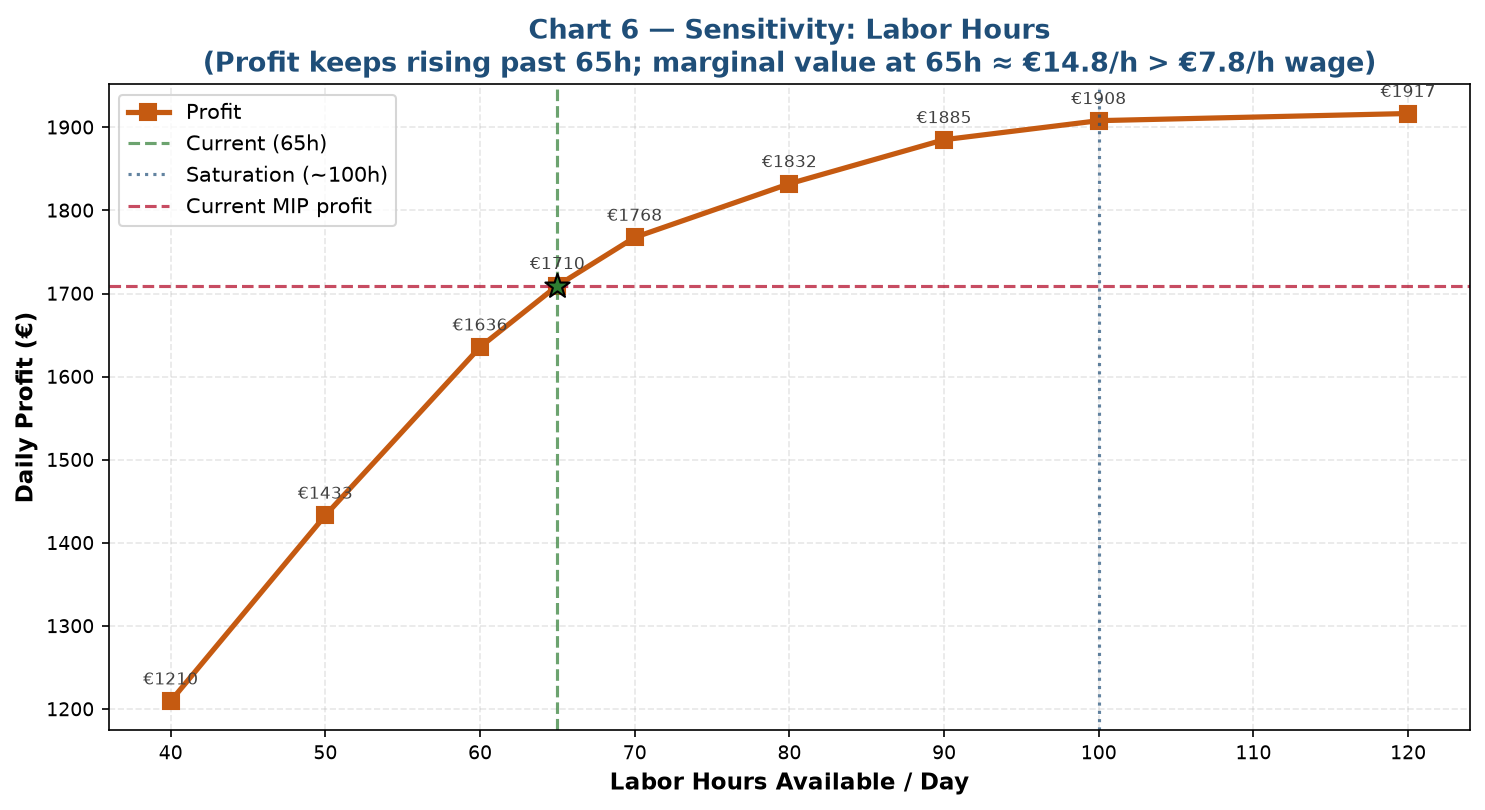
\includegraphics[width=0.78\textwidth]{chart_06_sensitivity_labor.png}
\caption{Κέρδος ως συνάρτηση των διαθέσιμων εργατοωρών. Η καμπύλη είναι αύξουσα με
φθίνον οριακό όφελος· ουσιαστικός κορεσμός γύρω στις $\sim 100$ ώρες (όχι στις 65).}
\label{fig:c7}
\end{figure}

\paragraph{Οικονομική ερμηνεία.} Το οριακό όφελος στο τρέχον σημείο ($H=65$) είναι
$\approx 14{,}8$\,€/ώρα — σχεδόν διπλάσιο του ωρομισθίου. Σε αντίθεση με μια βιαστική
ανάγνωση, η πρόσληψη επιπλέον προσωπικού είναι ξεκάθαρα κερδοφόρα: το κέρδος
συνεχίζει να αυξάνεται αρκετά πέρα από τις 65 ώρες και σταθεροποιείται γύρω στις
$\sim 100$ ώρες, όταν όλα τα επιλεγμένα πιάτα έχουν φτάσει τα όρια ζήτησής τους. Το
συμπέρασμα συμφωνεί απόλυτα με τη σκιώδη τιμή $u^\star=\LaborShadow$\,€/ώρα της
Ενότητας~\ref{sec:duality}.

\subsection{Ποσοστό σπατάλης (Σχήμα~\ref{fig:c8})}
Με μεταβολή του $\alpha$ από 0\% έως 20\%, το κέρδος πέφτει σχεδόν γραμμικά
(Πίνακας~\ref{tab:waste}, Σχήμα~\ref{fig:c8}). Κάθε ποσοστιαία μονάδα σπατάλης
κοστίζει περίπου 7,5\,€/ημέρα· η μείωση της σπατάλης από 6\% σε 3\% προσθέτει
$\approx 22{,}6$\,€/ημέρα (δηλ.\ $\sim 8000$\,€/έτος), δικαιολογώντας επενδύσεις σε
σωστή αποθήκευση και έλεγχο παρτίδων.

\begin{figure}[htbp]
\centering
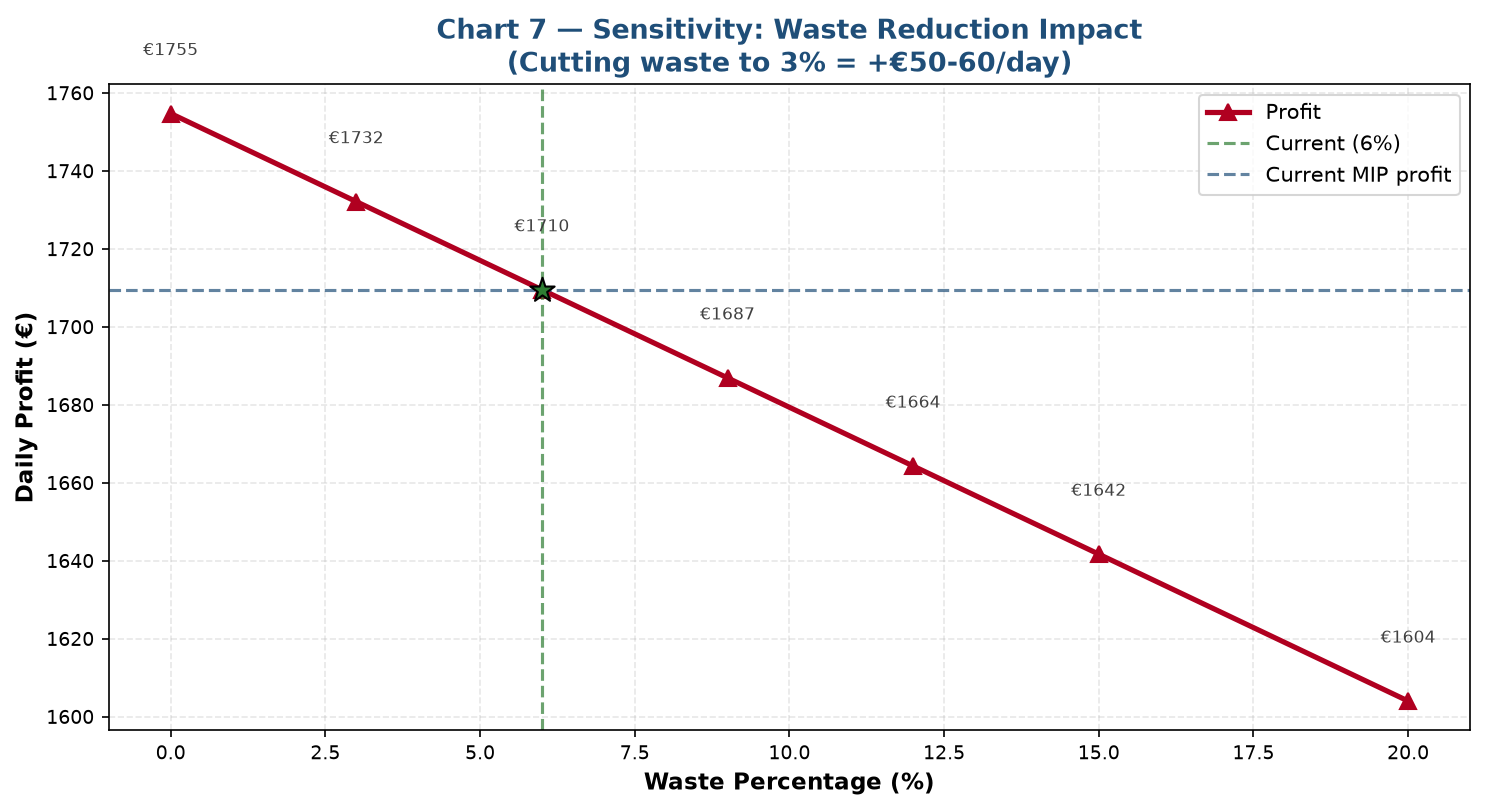
\includegraphics[width=0.78\textwidth]{chart_07_sensitivity_waste.png}
\caption{Επίδραση του ποσοστού σπατάλης $\alpha$ στο ημερήσιο κέρδος. Το αστέρι
σημειώνει το τρέχον επίπεδο (6\%).}
\label{fig:c8}
\end{figure}

\subsection{Μέγεθος μενού (όριο $N_{\max}$)}
Εφόσον το «10 πιάτα» είναι το ενεργό όριο $N_{\max}$, ο Πίνακας~\ref{tab:menu}
εξετάζει τι συμβαίνει με τη χαλάρωσή του. Παρατηρείται ότι η αύξηση του $N_{\max}$
αυξάνει το κέρδος με \emph{ισχυρά φθίνοντα} ρυθμό: το 11ο πιάτο προσθέτει μόλις
$\approx 8$\,€, ενώ η μετάβαση από 6 σε 10 πιάτα αυξάνει το κέρδος κατά
$\approx 467$\,€. Με τις τρέχουσες 65 ώρες, ένα μενού $\sim 10$ πιάτων είναι σχεδόν
βέλτιστο: επιπλέον πιάτα δεν αξίζουν τα πάγια κόστη τους εφόσον δεν υπάρχει επιπλέον
εργασία για να τα στηρίξει.

\begin{table}[htbp]
\centering
\caption{Ευαισθησία ως προς το μέγιστο μέγεθος μενού $N_{\max}$ (με $H=65$ ώρες).}
\label{tab:menu}
\small
\begin{tabular}{@{}lrr@{}}
\toprule
$N_{\max}$ & \textbf{Επιλεγμένα πιάτα} & \textbf{Κέρδος (€)} \\
\midrule
6 & 6 & 1242,52 \\
8 & 8 & 1535,65 \\
10 & 10 & 1709,53 \\
12 & 11 & 1717,41 \\
21 (χωρίς όριο) & 11 & 1717,41 \\
\bottomrule
\end{tabular}

\end{table}

% =====================================================================
\section{Συζήτηση: γιατί μένουν εκτός παραδοσιακά πιάτα;}\label{sec:discussion}
Εύλογο ερώτημα θα ήταν αν είναι ρεαλιστικό το μοντέλο να αφήνει εκτός μενού «κλασικά»
κερδοφόρα πιάτα όπως ο Μουσακάς ή το Γιουβέτσι. Η απάντηση, που η δυϊκή ανάλυση
κατέστησε πλέον \emph{αυστηρή}, απαιτεί προσοχή στη διατύπωση.

\paragraph{Δεν ισχύει ότι «ο μουσακάς δεν είναι κερδοφόρος».} Όπως προέκυψε στην
Ενότητα~\ref{sec:costing}, ο Μουσακάς έχει θετικό περιθώριο $m=4{,}44$\,€ ανά μερίδα.
Σε ένα εστιατόριο χωρίς περιορισμό χρόνου θα προσφερόταν ασφαλώς. Το ζήτημα είναι
αμιγώς \emph{κόστος ευκαιρίας}: όσο η εργασία είναι ο στενός πόρος, κάθε λεπτό που
αφιερώνεται στον Μουσακά (απόδοση 12,1\,€/ώρα) είναι ένα λεπτό που \emph{δεν}
αφιερώνεται στις Γαρίδες (50,5\,€/ώρα). Η δυϊκότητα το ποσοτικοποιεί ακριβώς: το
μειωμένο κόστος $r_{\text{μουσ.}}=-3{,}03$\,€ [σχέση~\eqref{eq:reduced}] είναι το
ημερήσιο κέρδος που θα χανόταν ανά επιβαλλόμενη μερίδα. Η ορθή διατύπωση είναι: όταν
η εργασία είναι σπάνια, τα χρονοβόρα πιάτα αποκλείονται όχι επειδή χάνουν χρήματα,
αλλά επειδή υπάρχουν πιο αποδοτικές χρήσεις του ίδιου χρόνου.

\paragraph{Επιβεβαίωση με πείραμα.} Η ανάλυση εργατοωρών (Ενότητα~\ref{sec:sensitivity})
έδειξε ότι η εργασία αξίζει να επεκταθεί. Με αύξηση του προσωπικού, η εικόνα για τα
παραδοσιακά πιάτα αλλάζει· επιλύοντας το \en{MIP} με άφθονη εργασία ($H=120$)
προκύπτει:
\begin{itemize}
  \item Με $N_{\max}=10$, ο \textbf{Μουσακάς επανέρχεται} στο βέλτιστο μενού.
  \item Με $N_{\max}=21$ (χωρίς ουσιαστικό όριο) επιλέγονται 16 πιάτα — \textbf{μαζί
  με το Γιουβέτσι} — και το κέρδος ανέρχεται σε $2596{,}77$\,€.
\end{itemize}
Με άλλα λόγια, τα «παραδοσιακά» πιάτα \emph{δεν} είναι εγγενώς ασύμφορα· απλώς έχουν
χαμηλότερη προτεραιότητα όταν ο χρόνος είναι περιορισμένος. Το ίδιο το μοντέλο, με
περισσότερη εργασία, τα επανεντάσσει στο μενού — εύρημα που συμφωνεί με τη διαπίστωση
ότι ο ανθρωποχρόνος μπορεί εύκολα να αυξηθεί κερδοφόρα.

\paragraph{Πρακτική σύσταση.} Συνδυαστικά, η στρατηγική σύσταση δεν είναι η μόνιμη
κατάργηση του Μουσακά, αλλά: στο \emph{τρέχον} επίπεδο δυναμικότητας προτεραιότητα
στα αποδοτικά ανά ώρα πιάτα· παράλληλα, εξέταση αύξησης προσωπικού (την οποία
δικαιολογεί η σκιώδης τιμή $u^\star=\LaborShadow$\,€/ώρα), οπότε τα κλασικά πιάτα
μπορούν να επανενταχθούν χωρίς θυσία κέρδους.

% =====================================================================
\section{Συμπεράσματα}\label{sec:conclusions}
\begin{enumerate}
  \item Αναπτύχθηκε ένα σύστημα δύο μοντέλων: το \en{LP} δίνει το \emph{άνω φράγμα}
  κέρδους ($1976{,}41$\,€), ενώ το \en{MIP} δίνει το \emph{υλοποιήσιμο} μενού
  ($1709{,}53$\,€, 10 πιάτα). Η διαφορά αναλύθηκε ποσοτικά [σχέση~\eqref{eq:decomp}]
  σε 241\,€ πάγιων κοστών και 26\,€ απώλειας ευελιξίας.
  \item Ο στενός πόρος είναι ο χρόνος προσωπικού· γι' αυτό το κρίσιμο μέτρο επιλογής
  είναι το περιθώριο \emph{ανά εργατοώρα} $\rho_d$, που υπολογίζεται απευθείας από τη
  βάση δεδομένων.
  \item Το πλήθος «10» των πιάτων αποτελεί το \emph{σχεδιαστικό} όριο $N_{\max}$ και
  όχι αυτόνομη ανακάλυψη του μοντέλου· η χαλάρωσή του αυξάνει το κέρδος με φθίνοντα
  ρυθμό.
  \item \textbf{Δυϊκή ανάλυση.} Επιβεβαιώθηκε αριθμητικά η ισχυρή
  δυϊκότητα ($Z^\star=W^\star=1976{,}41$\,€) και οι συνθήκες συμπληρωματικής
  χαλαρότητας. Η σκιώδης τιμή της εργασίας ($u^\star=\LaborShadow$\,€/ώρα)
  θεμελιώνει αυστηρά την κερδοφορία της πρόσληψης προσωπικού, ενώ τα μειωμένα κόστη
  ($r_{\text{μουσ.}}=-3{,}03$\,€) εξηγούν \emph{ποσοτικά} τον αποκλεισμό κάθε πιάτου
  ως κόστος ευκαιρίας.
  \item \textbf{Παραμετρική ανάλυση \& \en{branch \& bound}.} Η σκιώδης τιμή της
  εργασίας ισχύει σε πεπερασμένο εύρος $H\in[\Hlow,\Hhigh]$, και η επιτρεπτή αύξηση
  περιθωρίου κάθε αποκλειόμενου πιάτου ταυτίζεται με το μειωμένο κόστος του. Το
  διάκενο ακεραιότητας του \en{MIP} είναι μόλις $\IntGap$\,€ ($\IntGapPct\%$), με
  δύο μόνο κλασματικές μεταβλητές στη ρίζα του \en{branch \& bound}.
  \item Η ανάλυση ευαισθησίας ανέδειξε ότι (α)~το κόστος υλικών έχει τη μεγαλύτερη
  επίδραση, (β)~η μείωση σπατάλης αποδίδει σταθερά, και (γ)~η πρόσληψη προσωπικού
  είναι κερδοφόρα στο τρέχον επίπεδο — πλήρως συνεπές με τη δυϊκή σκιώδη τιμή.
  \item Τα παραδοσιακά χρονοβόρα πιάτα δεν είναι ασύμφορα· αποκλείονται λόγω κόστους
  ευκαιρίας και επανέρχονται μόλις αυξηθεί η διαθέσιμη εργασία — όπως επιβεβαιώθηκε
  πειραματικά.
\end{enumerate}

Το παραγόμενο σύστημα αποτελεί ένα ευέλικτο εργαλείο στρατηγικού σχεδιασμού: με
μεταβολή των παραμέτρων (ζήτηση, τιμές, εργατοώρες, μέγεθος μενού) ο διαχειριστής
λαμβάνει άμεσα το νέο βέλτιστο μενού μαζί με την οικονομική του τεκμηρίωση και,
πλέον, με πλήρη δυϊκή ερμηνεία της σπανιότητας κάθε πόρου.

% =====================================================================
\begin{thebibliography}{9}

\bibitem{silva} \en{Silva, A.\ et al., \textit{University restaurants menu planning
using mathematical modelling} (Integer Linear Programming).}
\url{https://www.cabidigitallibrary.org/doi/pdf/10.5555/20210125835}

\bibitem{razak} \en{Razak, N.\ A.\ et al., \textit{Application of Linear Programming
on Diet Problem for Kenny Roger's Roaster.}}
\url{https://oarep.usim.edu.my/bitstreams/be270cb5-54ea-46e6-9abf-1a1d9827174c/download}

\bibitem{sholeha} \en{Sholeha, M.\ et al., \textit{Diet-Menu Problem Modelling Based
on Linear Boolean Approach} (Boolean / Integer Linear Programming).}
\url{https://pubs.aip.org/aip/acp/article-pdf/doi/10.1063/5.0191844/20093229/060008_1_5.0191844.pdf}

\bibitem{stigler} \en{Stigler, G.\ J. (1945). \textit{The Cost of Subsistence.}
Journal of Farm Economics, 27(2), 303--314.}

\bibitem{dantzig} \en{Dantzig, G.\ B. (1963). \textit{Linear Programming and
Extensions.} Princeton University Press.}

\bibitem{bertsimas} \en{Bertsimas, D.\ \& Tsitsiklis, J.\ N. (1997).
\textit{Introduction to Linear Optimization.} Athena Scientific.} (Δυϊκότητα,
συμπληρωματική χαλαρότητα, ανάλυση ευαισθησίας.)

\bibitem{winston} \en{Winston, W.\ L. (2004). \textit{Operations Research:
Applications and Algorithms} (4th ed.). Thomson/Brooks-Cole.} (Ανάλυση εύρους /
\en{ranging}, σκιώδεις τιμές.)

\bibitem{landdoig} \en{Land, A.\ H.\ \& Doig, A.\ G. (1960). \textit{An Automatic
Method of Solving Discrete Programming Problems.} Econometrica, 28(3), 497--520.}
(Αρχική μέθοδος \en{branch \& bound}.)

\bibitem{wolsey} \en{Wolsey, L.\ A. (1998). \textit{Integer Programming.} Wiley.}
(Θεωρία ακέραιου προγραμματισμού, χαλαρώσεις, διάκενο ακεραιότητας.)

\bibitem{coincbc} \en{Forrest, J.\ et al. \textit{COIN-OR Branch-and-Cut (CBC)}·
Mitchell, S.\ et al. \textit{PuLP: A Linear Programming Toolkit for Python.}}
\url{https://github.com/coin-or/Cbc}

\end{thebibliography}

\end{document}
